% Created 2024-04-07 Κυρ 13:42
% Intended LaTeX compiler: pdflatex
\documentclass[11pt]{article}
\usepackage[utf8]{inputenc}
\usepackage[T1]{fontenc}
\usepackage{graphicx}
\usepackage{longtable}
\usepackage{wrapfig}
\usepackage{rotating}
\usepackage[normalem]{ulem}
\usepackage{amsmath}
\usepackage{amssymb}
\usepackage{capt-of}
\usepackage{hyperref}
\usepackage{booktabs}
\usepackage{import}
\usepackage[LGR, T1]{fontenc}
\usepackage[greek, english, american]{babel}
\usepackage{alphabeta}
\usepackage{esint}
\usepackage{mathtools}
\usepackage{esdiff}
\usepackage{makeidx}
\usepackage{glossaries}
\usepackage{newfloat}
\usepackage{minted}
\usepackage[a4paper, margin=3cm]{geometry}
\usepackage{chemfig}
\usepackage{svg}
\author{Vidianos Giannitsis}
\date{\today}
\title{Αποτελέσματα Αναερόβιας Χώνευσης σε BMPs}
\hypersetup{
 pdfauthor={Vidianos Giannitsis},
 pdftitle={Αποτελέσματα Αναερόβιας Χώνευσης σε BMPs},
 pdfkeywords={},
 pdfsubject={},
 pdfcreator={Emacs 29.3 (Org mode 9.6.15)}, 
 pdflang={English}}
\makeatletter
\newcommand{\citeprocitem}[2]{\hyper@linkstart{cite}{citeproc_bib_item_#1}#2\hyper@linkend}
\makeatother

\usepackage[notquote]{hanging}
\begin{document}

\maketitle
\tableofcontents

Σκοπός του αρχείου αυτού είναι η ανάλυση όλων των αποτελεσμάτων των διάφορων πειραμάτων αναερόβιας χώνευσης στην διάταξη για την εύρεση του biomethane potential. Θα αναλυθούν 3 βασικά πειράματα. Το πρώτο είναι η κινητική παραγωγής μεθανίου από οξικό οξύ, ενώ μετά θα αναλυθούν δύο πειράματα παραγωγής μεθανίου από το υδρόλυμα των αποβλήτων τροφών που παράχθηκε στο προηγούμενο στάδιο. Το αρχείο \url{./hplc\_analysis\_notebook.org} περιέχει τα αποτελέσματα των σχετικών πειραμάτων και αναφέρει τα πλεονεκτήματα και μειονεκτήματα τους.

\section{Dependencies}
\label{sec:org3246ff4}
Στο αρχείο αυτό θα οριστούν κάποια functions για να διευκολυνθεί η ανάλυση των BMPs, τα οποία θα είναι generic και μετά θα υπάρχουν κάποια specific code blocks για την εφαρμογή σε κάθε πείραμα. Πριν ξεκινήσουμε, κάνουμε activate το DrWatson project για reproducibility. Επίσης κάνουμε load το Dates.jl που θα χρειαστεί παρακάτω, καθώς και τα CSV.jl και DataFrames.jl που είναι πάντα χρήσιμα σε tabular data. Ακόμη, παρακάτω θα χρειαστούν τα LsqFit.jl για την προσαρμογή του μοντέλου Gompertz, StatsBase για υπολογισμό μέσων και Plots.jl για plotting. Το code block αυτό δεν κάνει tangle πουθενά καθώς είναι κομμάτι του generic code που θα χρησιμοποιηθεί σε πολλά σημεία.

\textbf{deps}
\begin{minted}[breaklines=true,breakanywhere=true]{julia}

using DrWatson
@quickactivate "Masters_Thesis"

using Dates
using StatsBase
using CSV, DataFrames
using LsqFit
using Plots

\end{minted}

\section{Acetate Experiment data reading}
\label{sec:orga9503df}
Τα δεδομένα της αναερόβιας χώνευσης είναι φωτογραφίες των προχωίδων της διάταξης. Εξετάζοντας πόσο έχει μεταβληθεί η στάθμη τους, μπορούμε να υπολογίσουμε τον παραγόμενο όγκο μεθανίου. Αλλά πρώτα, πρέπει να ξέρουμε σε τι χρόνους έγιναν sampled τα δείγματα. Όλες οι φωτογραφίες έχουν ένα timestamp το οποίο μας βοηθάει να τα διακρίνουμε. Μπορούμε να αναλύσουμε αυτά ώστε να πάρουμε τις στιγμές που βγήκαν οι φωτογραφίες. Αρχικά, παίρνουμε όλα τα filenames με \texttt{ls}. Θα χρησιμοποιήσουμε τα flags -m και -Q για να πάρουμε comma separated output και το κάθε string να έχει double quotes.

\textbf{ls\textsubscript{output}\textsubscript{acetate}}
\begin{minted}[breaklines=true,breakanywhere=true]{sh}
ls -mQ ../bmp_pictures/Acet_kinetics_screenshots/
\end{minted}

\begin{verbatim}
"bandicam 2024-03-27 18-45-55-857.jpg", "bandicam 2024-03-27 18-46-57-161.jpg",
"bandicam 2024-03-27 18-48-57-160.jpg", "bandicam 2024-03-27 18-50-57-170.jpg",
"bandicam 2024-03-27 18-52-57-164.jpg", "bandicam 2024-03-27 18-54-57-162.jpg",
"bandicam 2024-03-27 18-56-57-167.jpg", "bandicam 2024-03-27 18-58-57-165.jpg",
"bandicam 2024-03-27 19-00-57-170.jpg", "bandicam 2024-03-27 19-02-57-179.jpg",
"bandicam 2024-03-27 19-04-57-173.jpg", "bandicam 2024-03-27 19-06-57-182.jpg",
"bandicam 2024-03-27 19-08-57-185.jpg", "bandicam 2024-03-27 19-10-57-184.jpg",
"bandicam 2024-03-27 19-12-57-189.jpg", "bandicam 2024-03-27 19-14-57-187.jpg",
"bandicam 2024-03-27 19-15-06-279.jpg", "bandicam 2024-03-27 19-19-06-273.jpg",
"bandicam 2024-03-27 19-21-06-276.jpg", "bandicam 2024-03-27 19-23-06-285.jpg",
"bandicam 2024-03-27 19-25-06-290.jpg", "bandicam 2024-03-27 19-27-06-301.jpg",
"bandicam 2024-03-27 19-29-06-303.jpg", "bandicam 2024-03-27 19-31-06-301.jpg",
"bandicam 2024-03-27 19-33-06-297.jpg", "bandicam 2024-03-27 19-35-06-305.jpg",
"bandicam 2024-03-27 19-37-06-299.jpg", "bandicam 2024-03-27 19-39-06-297.jpg",
"bandicam 2024-03-27 19-41-06-307.jpg", "bandicam 2024-03-27 19-43-06-299.jpg",
"bandicam 2024-03-27 19-45-06-298.jpg", "bandicam 2024-03-27 19-47-06-304.jpg",
"bandicam 2024-03-27 19-48-50-591.jpg", "bandicam 2024-03-29 12-23-36-175.jpg",
"bandicam 2024-03-29 12-23-50-142.jpg", "bandicam 2024-03-29 12-24-50-161.jpg",
"bandicam 2024-03-29 12-25-50-156.jpg", "bandicam 2024-03-29 12-26-50-168.jpg",
"bandicam 2024-03-29 12-27-26-514.jpg", "bandicam 2024-03-29 12-28-26-502.jpg",
"bandicam 2024-03-29 12-29-26-497.jpg", "bandicam 2024-03-29 12-29-39-894.jpg",
"bandicam 2024-03-29 12-30-39-902.jpg", "bandicam 2024-03-29 12-31-39-897.jpg",
"bandicam 2024-03-29 12-32-05-844.jpg", "bandicam 2024-03-29 12-33-05-843.jpg",
"bandicam 2024-03-29 12-34-05-832.jpg", "bandicam 2024-03-29 12-35-05-836.jpg",
"bandicam 2024-03-29 12-36-05-835.jpg", "bandicam 2024-03-29 12-37-05-858.jpg",
"bandicam 2024-03-29 12-38-06-101.jpg", "bandicam 2024-03-29 12-38-47-045.jpg",
"bandicam 2024-03-29 12-39-47-039.jpg", "bandicam 2024-03-29 12-40-47-050.jpg",
"bandicam 2024-03-29 12-41-47-047.jpg", "bandicam 2024-03-29 12-42-47-057.jpg",
"bandicam 2024-03-29 12-43-42-169.jpg", "bandicam 2024-03-29 12-44-41-398.jpg"
\end{verbatim}

Αρχικά, κάνουμε load τα dependencies στο script στο οποίο θα γίνει η ανάλυση του πειράματος αυτού.

\begin{minted}[breaklines=true,breakanywhere=true]{julia}

<<deps>>

\end{minted}

Έπειτα, ξεκινάμε την ανάλυση αποθηκεύοντας τα file names σε ένα vector της Julia κάνοντας copy τα shell results. Αυτό το vector θα γίνεται loaded σε όλα τα code blocks, για να είναι το κάθε ένα reproducible από μόνο του. Έτσι, στο τελικό script θα υπάρχουν πολλές επαναλήψεις.

\textbf{date\textsubscript{saving}\textsubscript{acetate}}
\begin{minted}[breaklines=true,breakanywhere=true]{julia}

file_vec = ["bandicam 2024-03-27 18-45-55-857.jpg", "bandicam 2024-03-27 18-46-57-161.jpg",
"bandicam 2024-03-27 18-48-57-160.jpg", "bandicam 2024-03-27 18-50-57-170.jpg",
"bandicam 2024-03-27 18-52-57-164.jpg", "bandicam 2024-03-27 18-54-57-162.jpg",
"bandicam 2024-03-27 18-56-57-167.jpg", "bandicam 2024-03-27 18-58-57-165.jpg",
"bandicam 2024-03-27 19-00-57-170.jpg", "bandicam 2024-03-27 19-02-57-179.jpg",
"bandicam 2024-03-27 19-04-57-173.jpg", "bandicam 2024-03-27 19-06-57-182.jpg",
"bandicam 2024-03-27 19-08-57-185.jpg", "bandicam 2024-03-27 19-10-57-184.jpg",
"bandicam 2024-03-27 19-12-57-189.jpg", "bandicam 2024-03-27 19-14-57-187.jpg",
"bandicam 2024-03-27 19-15-06-279.jpg", "bandicam 2024-03-27 19-19-06-273.jpg",
"bandicam 2024-03-27 19-21-06-276.jpg", "bandicam 2024-03-27 19-23-06-285.jpg",
"bandicam 2024-03-27 19-25-06-290.jpg", "bandicam 2024-03-27 19-27-06-301.jpg",
"bandicam 2024-03-27 19-29-06-303.jpg", "bandicam 2024-03-27 19-31-06-301.jpg",
"bandicam 2024-03-27 19-33-06-297.jpg", "bandicam 2024-03-27 19-35-06-305.jpg",
"bandicam 2024-03-27 19-37-06-299.jpg", "bandicam 2024-03-27 19-39-06-297.jpg",
"bandicam 2024-03-27 19-41-06-307.jpg", "bandicam 2024-03-27 19-43-06-299.jpg",
"bandicam 2024-03-27 19-45-06-298.jpg", "bandicam 2024-03-27 19-47-06-304.jpg",
"bandicam 2024-03-27 19-48-50-591.jpg", "bandicam 2024-03-29 12-23-36-175.jpg",
"bandicam 2024-03-29 12-23-50-142.jpg", "bandicam 2024-03-29 12-24-50-161.jpg",
"bandicam 2024-03-29 12-25-50-156.jpg", "bandicam 2024-03-29 12-26-50-168.jpg",
"bandicam 2024-03-29 12-27-26-514.jpg", "bandicam 2024-03-29 12-28-26-502.jpg",
"bandicam 2024-03-29 12-29-26-497.jpg", "bandicam 2024-03-29 12-29-39-894.jpg",
"bandicam 2024-03-29 12-30-39-902.jpg", "bandicam 2024-03-29 12-31-39-897.jpg",
"bandicam 2024-03-29 12-32-05-844.jpg", "bandicam 2024-03-29 12-33-05-843.jpg",
"bandicam 2024-03-29 12-34-05-832.jpg", "bandicam 2024-03-29 12-35-05-836.jpg",
"bandicam 2024-03-29 12-36-05-835.jpg", "bandicam 2024-03-29 12-37-05-858.jpg",
"bandicam 2024-03-29 12-38-06-101.jpg", "bandicam 2024-03-29 12-38-47-045.jpg",
"bandicam 2024-03-29 12-39-47-039.jpg", "bandicam 2024-03-29 12-40-47-050.jpg",
"bandicam 2024-03-29 12-41-47-047.jpg", "bandicam 2024-03-29 12-42-47-057.jpg",
"bandicam 2024-03-29 12-43-42-169.jpg", "bandicam 2024-03-29 12-44-41-398.jpg"
]

\end{minted}

\section{FW Hydrolysate Experiment 1 Data Reading}
\label{sec:org012e73d}
Με την ίδια λογική με παραπάνω, κάνουμε load ότι θα χρειαστεί για αυτό το πείραμα.

\textbf{ls\textsubscript{output}\textsubscript{fw}\textsubscript{1}}
\begin{minted}[breaklines=true,breakanywhere=true]{sh}
ls -mQ ../bmp_pictures/Hydrolyzed_FW_1/
\end{minted}

\begin{minted}[breaklines=true,breakanywhere=true]{julia}

<<deps>>

\end{minted}

\begin{minted}[breaklines=true,breakanywhere=true]{julia}

file_vec = ["bandicam 2024-04-01 11-05-53-069.jpg", "bandicam 2024-04-01 11-09-37-035.jpg",
"bandicam 2024-04-01 11-11-37-051.jpg", "bandicam 2024-04-01 11-12-37-060.jpg",
"bandicam 2024-04-01 11-13-26-776.jpg", "bandicam 2024-04-01 11-14-26-770.jpg",
"bandicam 2024-04-01 11-15-26-780.jpg", "bandicam 2024-04-01 11-21-53-098.jpg",
"bandicam 2024-04-01 11-52-12-665.jpg", "bandicam 2024-04-01 12-22-12-663.jpg",
"bandicam 2024-04-01 16-52-12-699.jpg", "bandicam 2024-04-02 10-54-01-344.jpg",
"bandicam 2024-04-02 12-54-01-788.jpg", "bandicam 2024-04-02 13-24-01-783.jpg",
"bandicam 2024-04-02 13-54-01-797.jpg", "bandicam 2024-04-02 14-24-01-798.jpg",
"bandicam 2024-04-02 14-54-01-793.jpg", "bandicam 2024-04-02 15-24-01-786.jpg",
"bandicam 2024-04-02 15-54-01-785.jpg", "bandicam 2024-04-02 16-24-01-800.jpg",
"bandicam 2024-04-02 16-54-01-801.jpg", "bandicam 2024-04-02 17-24-01-784.jpg",
"bandicam 2024-04-02 17-54-02-191.jpg", "bandicam 2024-04-02 19-54-02-222.jpg",
"bandicam 2024-04-02 21-54-02-318.jpg", "bandicam 2024-04-02 23-54-02-573.jpg",
"bandicam 2024-04-03 01-54-02-576.jpg", "bandicam 2024-04-03 03-54-02-564.jpg",
"bandicam 2024-04-03 05-54-02-863.jpg", "bandicam 2024-04-03 07-54-02-978.jpg",
"bandicam 2024-04-03 09-54-02-983.jpg", "bandicam 2024-04-03 12-54-03-516.jpg",
"bandicam 2024-04-03 13-54-03-505.jpg", "bandicam 2024-04-03 14-24-03-564.jpg"
]
\end{minted}

\section{Data Processing}
\label{sec:org965d83e}
Έπειτα, μπορούμε να κάνουμε extract τις πληροφορίες που θέλουμε, με το Dates.jl package της Julia. Σε αυτό το code block, δεν θα ορίσουμε το file vector και αυτό θα υποτεθεί defined. Έτσι, δεν μπορούμε να τρέξουμε independently το block αυτό, αλλά μόνο chained σε ένα definition των files, για να μπορεί να τρέξει αντίστοιχα σε κάθε πείραμα. Επίσης, εκτός από να κάνουμε extract τα time stamps, φτιάχνουμε και ένα δεύτερο vector με time stamp dd/mm\textsubscript{HH}:MM το οποίο είναι πιο βολικό στη χρήση για εμένα.

Στη συνέχεια, ορίζουμε άλλη μία μεταβλητή η οποία δεν υπάρχει, η \texttt{inds}. Αυτή είναι τα νούμερα στο date\textsubscript{vec} που αντιστοιχούν σε ένα ορισμένο πείραμα. Παίρνουμε τα time stamps και στην αρχική αλλά και στην formatted μορφή για αυτό το πείραμα και μετά υπολογίζουμε τα time steps και σε δευτερόλεπτα αλλά και σε λεπτά. Η αφαίρεση δύο \texttt{DateTime} objects δίνει αποτέλεσμα σε \texttt{Millisecond}, οπότε ο χρόνος σε δευτερόλεπτα διαιρεί με 1000 \texttt{Millisecond} ενώ σε λεπτά με 60000 \texttt{Millisecond}. Έπειτα, ορίζουμε ένα τρίτο undefined variable το exp\textsubscript{meth}\textsubscript{vol}, το οποίο είναι η παραγωγή μεθανίου μεταξύ των δύο φωτογραφιών, όπως σημειώνεται σε αυτές. Για την κινητική, θέλουμε την αθροιστική παραγωγή μεθανίου, οπότε χρησιμοποιούμε την συνάρτηση \texttt{cumsum}.

Τέλος, αποθηκεύουμε όλα αυτά τα δεδομένα σε ένα table του \texttt{Tables.jl} interface, ώστε να μπορούμε να το κάνουμε DataFrame με headers για καλύτερο readability ή να το κάνουμε export σε csv. Για το csv export χρειαζόμαστε ένα file name. Αυτό μπορεί για άλλη μία φορά να μην οριστεί εδώ και να χρησιμοποιηθεί ως variable. Βέβαια, ένα σημαντικό σημείο είναι πως τα πειράματα με οξικό πάνε γρήγορα, ενώ με το υδρόλυμα των FW αρκετά πιο αργά. Οπότε, αν το variable \texttt{source} είναι ίσο με "Hydrolyzed FW", κάνουμε save τον χρόνο σε λεπτά και ώρες, αλλιώς σε λεπτά και δευτερόλεπτα.

\textbf{bmp\textsubscript{data}\textsubscript{processing}}
\begin{minted}[breaklines=true,breakanywhere=true]{julia}

date_vec = [DateTime(SubString(file_vec[i], 10, 32), "yyyy-mm-dd HH-MM-SS-sss") for i in 1:length(file_vec)]
formatted_date = [Dates.format(date_vec[i], "dd/mm_HH:MM") for i in 1:length(date_vec)]

exp_stamps = date_vec[inds]
exp_formatted = formatted_date[inds]
exp_sec = round.([(exp_stamps[i] - exp_stamps[1])/Millisecond(1000) for i in 1:length(inds)]; digits = 4)
exp_min = round.([(exp_stamps[i] - exp_stamps[1])/Millisecond(60000) for i in 1:length(inds)]; digits = 4)
exp_hour = round.([(exp_stamps[i] - exp_stamps[1])/Millisecond(3600000) for i in 1:length(inds)]; digits = 4)
exp_cum_meth_vol = round.(cumsum(exp_meth_vol); digits = 3)

if source == "Acetate"
    exp_data = Tables.table(hcat(exp_formatted, exp_sec, exp_min, exp_meth_vol, exp_cum_meth_vol), header = [:Timestamp, :Seconds, :Minutes, :Methane_Volume, :Cumulative_Methane_Volume])
else
    exp_data = Tables.table(hcat(exp_formatted, exp_min, exp_hour, exp_meth_vol, exp_cum_meth_vol), header = [:Timestamp, :Minutes, :Hours, :Methane_Volume, :Cumulative_Methane_Volume])
end

CSV.write(datadir("exp_pro", exp_name*".csv"), exp_data)
exp_df = DataFrame(exp_data)

\end{minted}

\subsection{Curve Fitting}
\label{sec:org0f58436}
Επίσης, θέλουμε να κάνουμε fit τα δεδομένα σε κάποιο κινητικό μοντέλο για την διεργασία, κάτι το οποίο θα βοηθήσει στη μοντελοποιήση της. Το μοντέλο Gompertz είναι ένα μοντέλο που χρησιμοποιείται συχνά για kinetic modelling διεργασιών όπως η παραγωγή μεθανίου μέσω αναερόβιας χώνευσης, οπότε θα χρησιμοποιηθεί αυτό. Η εξίσωση που θα πρέπει να προσαρμοστεί είναι η
\[ P(t) = P_{\max } \exp \left( - \exp \left[ \frac{R_{\max }e (λ-t)}{P_{\max }} + 1 \right] \right) \]
όπου P(t) η παραγωγή μεθανίου την στιγμή t, P\textsubscript{max} η μέγιστη ποσότητα μεθανίου που μπορεί να παραχθεί από το υπόστρωμα αυτό, R\textsubscript{max} ο ειδικός ρυθμός παραγωγής μεθανίου, λ το lag time και e η σταθερά Euler. Παρακάτω φαίνεται το fit των δεδομένων στην συνάρτηση αυτή. Αξίζει να αναφερθεί η χρήση της μεταβλητής \texttt{input\_cod} που φαίνεται παρακάτω. Η μεταβλητή αυτή εκφράζει το COD της τροφοδοσίας. Διαιρούμε τον όγκο μεθανίου με αυτήν ώστε το διάγραμμα να εκφράζει ειδικό ρυθμό παραγωγής μεθανίου σε \(\frac{\text{mL CH$_4$}}{\text{g sCOD}}\), το οποίο είναι πιο εύκολα συγκρίσιμο με βιβλιογραφία, σε σχέση με τον όγκο μεθανίου. Επίσης, αξίζει να σημειωθεί η χρήση bounded optimization. Οι παραμέτροι του μοντέλου έχουν νόημα μόνο ως θετικοί αριθμοί. Στα πειράματα με χρήση οξικό ως υπόστρωμα, όπου οι μικροοργανισμοί αντιδρούν ταχύτατα στην αλλαγή του περιβάλλοντος, η προσαρμογή του μοντέλου έδινε αρνητικό lag time. Αυτό προφανώς δεν έχει νόημα και στην πράξη, το συμπέρασμα είναι πως το lag time είναι μηδενικό (σχεδόν ακαριαία αντίδραση των μικροοργανισμών στην προσθήκη οξικού στο σύστημα). Επίσης, αξίζει να αναφερθεί η μεταβλητή \texttt{kinetics}. Σε κάποια πειράματα (πχ τις μετρήσεις παραγωγής μεθανίου χωρίς προσθήκη υποστρώματος που έγινε σε ένα δείγμα) δεν θέλουμε να κάνουμε προσαρμογή με το μοντέλο Gompertz. Αυτή η μεταβλητή είναι στην ουσία ένα toggle off του plot με την κινητική, για όσα πειράματα δεν το χρειάζονται.

Παρακάτω υπάρχουν 2 code blocks. Το πρώτο κάνει fit σε timescale λεπτών ενώ το δεύτερο σε ωρών. Ανάλογα με το πείραμα, μπορεί να βγάλουν ίδια αποτελέσματα, αλλά ενδέχεται να είναι και διαφορετικά.

\textbf{bmp\textsubscript{curve}\textsubscript{fitting}\textsubscript{min}}
\begin{minted}[breaklines=true,breakanywhere=true]{julia}

gompertz(t, p) = @. p[1]*exp(-exp((((p[2]*exp(1))/p[1])*(p[3] - t)) + 1))

lb = [0.0, 0.0, 0.0]
ub = [Inf, Inf, Inf]
specific_meth_vol = exp_cum_meth_vol./input_cod

fit = curve_fit(gompertz, exp_min, specific_meth_vol, p0, lower = lb, upper = ub)

model_params = fit.param
gompertz(t) = gompertz(t, model_params)

model_res = fit.resid
SS_res = sum(model_res.^2)
SS_tot = sum([(specific_meth_vol[i] - mean(specific_meth_vol)).^2 for i in 1:length(specific_meth_vol)])
r_squared = 1 - SS_res/SS_tot

kinetics = true
timescale = "min"
\end{minted}


\textbf{bmp\textsubscript{curve}\textsubscript{fitting}\textsubscript{hour}}
\begin{minted}[breaklines=true,breakanywhere=true]{julia}

gompertz(t, p) = @. p[1]*exp(-exp((((p[2]*exp(1))/p[1])*(p[3] - t)) + 1))
lb = [0.0, 0.0, 0.0]
ub = [Inf, Inf, Inf]
specific_meth_vol = exp_cum_meth_vol./input_cod

fit = curve_fit(gompertz, exp_hour, specific_meth_vol, p0, lower = lb, upper = ub)

model_params = fit.param
gompertz(t) = gompertz(t, model_params)

model_res = fit.resid
SS_res = sum(model_res.^2)
SS_tot = sum([(specific_meth_vol[i] - mean(specific_meth_vol)).^2 for i in 1:length(specific_meth_vol)])
r_squared = 1 - SS_res/SS_tot

kinetics = true
timescale = "hour"
\end{minted}

\subsection{Plotting}
\label{sec:org95392cb}
Τέλος, έχοντας προσαρμώσει το μοντέλο Gompertz σε κάθε σετ δεδομένων, θέλουμε να φτιάξουμε κάποια διαγράμματα με τα δεδομένα, τα οποία να δείχνουν την παραγόμενη ποσότητα μεθανίου στον χρόνο. Τα πειραματικά δεδομένα θα γίνουν plotted σε scatter plots. Χάριν ευκολίας, μπορούν να γίνουν plotted διαγράμματα και της στιγμιαίας αλλά και της συνολικής παραγωγής μεθανίου και σε άξονα χρόνου είτε λεπτά ή δευτερόλεπτα. Ο παραπάνω κώδικας υπολογίζει το fit του cumulative methane production σε λεπτά, καθώς θεωρείται η πιο χρήσιμη έκφραση, οπότε αυτό θα είναι και το διάγραμμα που έχει fit την καμπύλη. Εδώ θα εκμεταλλευτούμε τα variables που υπολογίζονται παραπάνω καθώς και 2 ακόμη, το \texttt{sample} και το \texttt{source}. Το \texttt{source} είναι ένα απλό variable το οποίο εκφράζει αν η τροφοδοσία ήταν οξικό ή υδρόλυμα για να τα ξεχωρίζουμε πιο εύκολα. Επίσης, χρησιμοποιείται για να κάνει generate τα σωστά plots (δευτερόλεπτα και λεπτά με fitting σε λεπτά για οξικό, λεπτά και ώρες με fitting ανάλογα το timescale για τα υδρολύματα). Το \texttt{sample} εκφράζει το νούμερο του δείγματος για να είναι πιο εύκολο το naming scheme.

\textbf{bmp\textsubscript{data}\textsubscript{plotting}}
\begin{minted}[breaklines=true,breakanywhere=true]{julia}

if source == "Acetate"
    bmp_cumulative_scatter_min = scatter(exp_min, exp_cum_meth_vol, markersize = 5, legend = false, xlabel = "Time (min)", ylabel = "Cumulative Methane Volume (mL)", title = "Cumulative Methane Production from "*source*" - "*sample, size = (700, 470))
    savefig(bmp_cumulative_scatter_min, plotsdir("BMPs", source, "cumulative_"*exp_name*"_min.png"))

    bmp_cumulative_scatter_sec = scatter(exp_sec, exp_cum_meth_vol, markersize = 5, legend = false, xlabel = "Time (sec)", ylabel = "Cumulative Methane Volume (mL)", title = "Cumulative Methane Production from "*source*" - "*sample, size = (700, 470))
    savefig(bmp_cumulative_scatter_sec, plotsdir("BMPs", source, "cumulative_"*exp_name*"_sec.png"))

    if kinetics
        bmp_specific_methane = scatter(exp_min, specific_meth_vol, markersize = 5, label = "Experimental Data", xlabel = "Time (min)", ylabel = "Cumulative Methane Production (mL/g sCOD)", title = "Methane Production Kinetics from "*source*" - "*sample, size = (700, 470), legend = :bottomright)
        plot!(exp_min, gompertz(exp_min), label = "Gompertz Model with R^2 = "*string(round(r_squared, digits = 3)))
        savefig(bmp_specific_methane, plotsdir("BMPs", source, "methane_kinetics_"*exp_name*".png"))
    end
else
    bmp_cumulative_scatter_min = scatter(exp_min, exp_cum_meth_vol, markersize = 5, legend = false, xlabel = "Time (min)", ylabel = "Cumulative Methane Volume (mL)", title = "Cumulative Methane Production from "*source*" - "*sample, size = (700, 470))
    savefig(bmp_cumulative_scatter_min, plotsdir("BMPs", source, "cumulative_"*exp_name*"_min.png"))

    bmp_cumulative_scatter_hour = scatter(exp_hour, exp_cum_meth_vol, markersize = 5, legend = false, xlabel = "Time (hour)", ylabel = "Cumulative Methane Volume (mL)", title = "Cumulative Methane Production from "*source*" - "*sample, size = (700, 470))
    savefig(bmp_cumulative_scatter_hour, plotsdir("BMPs", source, "cumulative_"*exp_name*"_hour.png"))

    if timescale == "hour"
        bmp_specific_methane = scatter(exp_hour, specific_meth_vol, markersize = 5, label = "Experimental Data", xlabel = "Time (hour)", ylabel = "Cumulative Methane Production (mL/g sCOD)", title = "Methane Production Kinetics from "*source*" - "*sample, size = (700, 470), legend = :bottomright)
        plot!(exp_hour, gompertz(exp_hour), label = "Gompertz Model with R^2 = "*string(round(r_squared, digits = 3)))
        savefig(bmp_specific_methane, plotsdir("BMPs", source, "methane_kinetics_"*exp_name*"_"*timescale*".png"))
    elseif timescale =="min" 
        bmp_specific_methane = scatter(exp_min, specific_meth_vol, markersize = 5, label = "Experimental Data", xlabel = "Time (min)", ylabel = "Cumulative Methane Production (mL/g sCOD)", title = "Methane Production Kinetics from "*source*" - "*sample, size = (700, 470), legend = :bottomright)
        plot!(exp_min, gompertz(exp_min), label = "Gompertz Model with R^2 = "*string(round(r_squared, digits = 3)))
        savefig(bmp_specific_methane, plotsdir("BMPs", source, "methane_kinetics_"*exp_name*"_"*timescale*".png"))
    end
end

\end{minted}

\section{Acetate Experiment Processing}
\label{sec:org8ebf262}
Παρακάτω αναφέρονται οι δοκιμές που έγιναν με 100 μL οξικό σε κάθε δείγμα και θα χρησιμοποιηθούν πιθανόν συγκριτικά σε σχέση με τα FW. Μετά από τα code blocks που τρέχουν τον κώδικα θα υπάρχουν και κάποια από τα corresponding αποτελέσματα. Συγκεκριμένα, ο πίνακας με τα κινητικά δεδομένα, το διάγραμμα παραγωγής μεθανίου το οποίο έχει το curve fitting και το διάγραμμα στιγμίαιας παραγωγής μεθανίου. Υπάρχουν και κάποια άλλα χρήσιμα διαγράμματα, τα οποία είναι αποθηκευμένα, αλλά εδώ παρατίθενται κάποια για καλύτερη ανάγνωση του αρχείου.

\subsection{Acetate Test FW}
\label{sec:org7289072}
Το section αυτό αναφέρεται στη δοκιμή με 100 μL οξικό στο δείγμα labelled ως FW (στο οποίο θα τροφοδοτηθούν untreated FW). Notably, δεν είχε διαρροή στις 27/03, αλλά για κάποιον λόγο, στην επαναδοκιμή στις 29/03 δεν παρήγαγε μεθάνιο (τουλάχιστον στην προχοίδα). Οπότε, θα χρησιμοποιηθεί αυτό της 27/03.

\textbf{acet\textsubscript{test}\textsubscript{FW}}
\begin{minted}[breaklines=true,breakanywhere=true]{julia}

### Data Analysis on Sample FW ###

<<date_saving_acetate>>

inds = 1:12
exp_meth_vol = [0, 12, 5, 3, 1.5, 1.5, 1, 1.5, 1, 0.5, 0.5, 0.5]
exp_name = "acet_test_fw"
source = "Acetate"
sample = "Sample FW"
input_cod = 0.1
p0 = [250.0, 60.0, 1.0]

<<bmp_data_processing>>
<<bmp_curve_fitting_min>>
model_acet_fw = vcat(sample, model_params, r_squared)
<<bmp_data_plotting>>
\end{minted}

\begin{table}[htbp]
\caption{Κινητικά δεδομένα}
\centering
\begin{tabular}{lrrrr}
Timestamp & Seconds & Minutes & Methane\textsubscript{Volume} & Cumulative\textsubscript{Methane}\textsubscript{Volume}\\[0pt]
\hline
27/03\textsubscript{18}:45 & 0.0 & 0.0 & 0.0 & 0.0\\[0pt]
27/03\textsubscript{18}:46 & 61.304 & 1.02173 & 12.0 & 12.0\\[0pt]
27/03\textsubscript{18}:48 & 181.303 & 3.02172 & 5.0 & 17.0\\[0pt]
27/03\textsubscript{18}:50 & 301.313 & 5.02188 & 3.0 & 20.0\\[0pt]
27/03\textsubscript{18}:52 & 421.307 & 7.02178 & 1.5 & 21.5\\[0pt]
27/03\textsubscript{18}:54 & 541.305 & 9.02175 & 1.5 & 23.0\\[0pt]
27/03\textsubscript{18}:56 & 661.31 & 11.0218 & 1.0 & 24.0\\[0pt]
27/03\textsubscript{18}:58 & 781.308 & 13.0218 & 1.5 & 25.5\\[0pt]
27/03\textsubscript{19}:00 & 901.313 & 15.0219 & 1.0 & 26.5\\[0pt]
27/03\textsubscript{19}:02 & 1021.322 & 17.0220 & 0.5 & 27.0\\[0pt]
27/03\textsubscript{19}:04 & 1141.316 & 19.0219 & 0.5 & 27.5\\[0pt]
27/03\textsubscript{19}:06 & 1261.325 & 21.0220 & 0.5 & 28.0\\[0pt]
\end{tabular}
\end{table}

\begin{center}
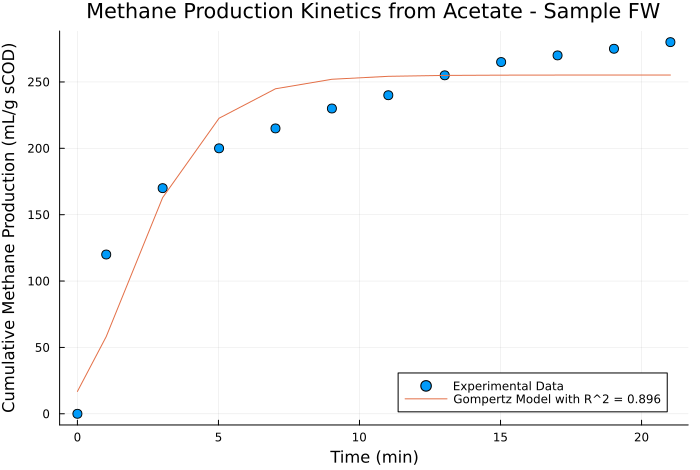
\includegraphics[width=.9\linewidth]{../plots/BMPs/Acetate/methane_kinetics_acet_test_fw.png}
\end{center}

\subsection{Acetate Test 0}
\label{sec:orgc7418b0}
Το section αυτό αναφέρεται στη δοκιμή με 100 μL οξικό στο δείγμα (0).

\textbf{acet\textsubscript{test}\textsubscript{0}}
\begin{minted}[breaklines=true,breakanywhere=true]{julia}

### Data Analysis on Sample 0 ###

<<date_saving_acetate>>

inds = 34:51
exp_meth_vol = [0, 4, 12, 7.5, 4.5, 2.5, 2.5, 4, 0.5, 2, 2, 1, 1, 1, 1, 1, 0.5, 0.5]
exp_name = "acet_test_0"
source = "Acetate"
sample = "Sample 0"
input_cod = 0.1
p0 = [400.0, 80.0, 1.0]

<<bmp_data_processing>>
<<bmp_curve_fitting_min>>
model_acet_0 = vcat(sample, model_params, r_squared)
<<bmp_data_plotting>>
\end{minted}

\begin{table}[htbp]
\caption{Κινητικά δεδομένα}
\centering
\begin{tabular}{lrrrr}
Timestamp & Seconds & Minutes & Methane\textsubscript{Volume} & Cumulative\textsubscript{Methane}\textsubscript{Volume}\\[0pt]
\hline
29/03\textsubscript{12}:23 & 0.0 & 0.0 & 0.0 & 0.0\\[0pt]
29/03\textsubscript{12}:23 & 13.967 & 0.2327 & 4.0 & 4.0\\[0pt]
29/03\textsubscript{12}:24 & 73.986 & 1.2331 & 12.0 & 16.0\\[0pt]
29/03\textsubscript{12}:25 & 133.981 & 2.2330 & 7.5 & 23.5\\[0pt]
29/03\textsubscript{12}:26 & 193.993 & 3.2332 & 4.5 & 28.0\\[0pt]
29/03\textsubscript{12}:27 & 230.339 & 3.8389 & 2.5 & 30.5\\[0pt]
29/03\textsubscript{12}:28 & 290.327 & 4.8388 & 2.5 & 33.0\\[0pt]
29/03\textsubscript{12}:29 & 350.322 & 5.8387 & 4.0 & 37.0\\[0pt]
29/03\textsubscript{12}:29 & 363.719 & 6.0619 & 0.5 & 37.5\\[0pt]
29/03\textsubscript{12}:30 & 423.727 & 7.0621 & 2.0 & 39.5\\[0pt]
29/03\textsubscript{12}:31 & 483.722 & 8.0620 & 2.0 & 41.5\\[0pt]
29/03\textsubscript{12}:32 & 509.669 & 8.4945 & 1.0 & 42.5\\[0pt]
29/03\textsubscript{12}:33 & 569.668 & 9.4945 & 1.0 & 43.5\\[0pt]
29/03\textsubscript{12}:34 & 629.657 & 10.4943 & 1.0 & 44.5\\[0pt]
29/03\textsubscript{12}:35 & 689.661 & 11.4943 & 1.0 & 45.5\\[0pt]
29/03\textsubscript{12}:36 & 749.66 & 12.4943 & 1.0 & 46.5\\[0pt]
29/03\textsubscript{12}:37 & 809.683 & 13.4947 & 0.5 & 47.0\\[0pt]
29/03\textsubscript{12}:38 & 869.926 & 14.4987 & 0.5 & 47.5\\[0pt]
\end{tabular}
\end{table}

\begin{center}
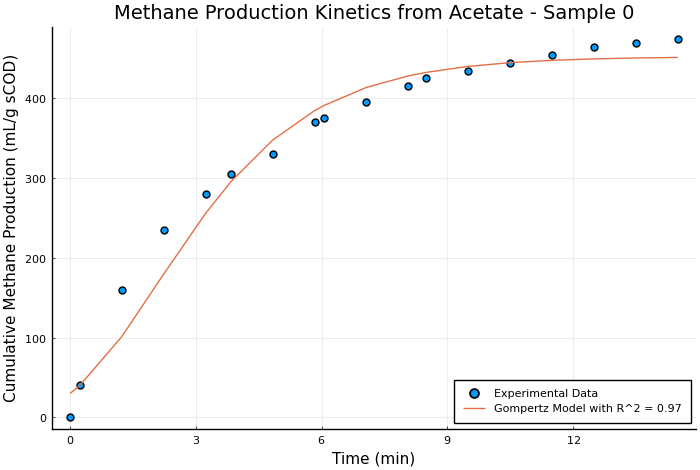
\includegraphics[width=.9\linewidth]{../plots/BMPs/Acetate/methane_kinetics_acet_test_0.png}
\end{center}

\subsection{Acetate Test 1}
\label{sec:orgcb55445}
Το section αυτό αναφέρεται στη δοκιμή με 100 μL οξικό στο δείγμα (1). Aξίζει να αναφερθεί πως την πρώτη πειραματική ημέρα (27/03), παρήγαγε αέριο χωρίς να τροφοδοτηθεί με κάποιο υπόστρωμα. Η κινητική αυτής της παραγωγής (η οποία δεν ξέρουμε σε τι ευθύνεται) θα αναλυθεί παρακάτω. Βέβαια, μόλις τροφοδοτήθηκε με οξικό και η παραγωγή του τελείωσε, σταμάτησε και εκείνη η παραγωγή. Βέβαια, είχε την χαμηλότερη παραγωγή βιοαερίου μόλις τροφοδοτήθηκε με οξικό, οπότε ενδέχεται αυτή η μέτρηση να ήταν προβληματική.

\textbf{acet\textsubscript{test}\textsubscript{1}}
\begin{minted}[breaklines=true,breakanywhere=true]{julia}

### Data Analysis on Sample 1 ###

<<date_saving_acetate>>

inds = 38:56
exp_meth_vol = [0, 6.5, 5, 3, 0.5, 1.5, 1.5, 0.5, 1, 0.5, 0.5, 0.3, 0.2, 0.2, 0.1, 0.05, 0.05, 0.05, 0.05]
exp_name = "acet_test_1"
source = "Acetate"
sample = "Sample 1"
input_cod = 0.1
p0 = [200.0, 40.0, 1.0]

<<bmp_data_processing>>
<<bmp_curve_fitting_min>>
model_acet_1 = vcat(sample, model_params, r_squared)
<<bmp_data_plotting>>
\end{minted}

\begin{verbatim}
sys:1: UserWarning: No data for colormapping provided via 'c'. Parameters 'vmin', 'vmax' will be ignored
sys:1: UserWarning: No data for colormapping provided via 'c'. Parameters 'vmin', 'vmax' will be ignored
sys:1: UserWarning: No data for colormapping provided via 'c'. Parameters 'vmin', 'vmax' will be ignored
"/home/vidianos/Documents/9o_εξάμηνο/Masters_Thesis/plots/BMPs/Acetate/methane_kinetics_acet_test_1.png"
\end{verbatim}


\begin{table}[htbp]
\caption{Κινητικά δεδομένα}
\centering
\begin{tabular}{lrrrr}
Timestamp & Seconds & Minutes & Methane\textsubscript{Volume} & Cumulative\textsubscript{Methane}\textsubscript{Volume}\\[0pt]
\hline
29/03\textsubscript{12}:26 & 0.0 & 0.0 & 0.0 & 0.0\\[0pt]
29/03\textsubscript{12}:27 & 36.346 & 0.6058 & 6.5 & 6.5\\[0pt]
29/03\textsubscript{12}:28 & 96.334 & 1.6055 & 5.0 & 11.5\\[0pt]
29/03\textsubscript{12}:29 & 156.329 & 2.6055 & 3.0 & 14.5\\[0pt]
29/03\textsubscript{12}:29 & 169.726 & 2.8288 & 0.5 & 15.0\\[0pt]
29/03\textsubscript{12}:30 & 229.734 & 3.8289 & 1.5 & 16.5\\[0pt]
29/03\textsubscript{12}:31 & 289.729 & 4.8288 & 1.5 & 18.0\\[0pt]
29/03\textsubscript{12}:32 & 315.676 & 5.2613 & 0.5 & 18.5\\[0pt]
29/03\textsubscript{12}:33 & 375.675 & 6.2612 & 1.0 & 19.5\\[0pt]
29/03\textsubscript{12}:34 & 435.664 & 7.2610 & 0.5 & 20.0\\[0pt]
29/03\textsubscript{12}:35 & 495.668 & 8.2611 & 0.5 & 20.5\\[0pt]
29/03\textsubscript{12}:36 & 555.667 & 9.2611 & 0.3 & 20.8\\[0pt]
29/03\textsubscript{12}:37 & 615.69 & 10.2615 & 0.2 & 21.0\\[0pt]
29/03\textsubscript{12}:38 & 675.933 & 11.2655 & 0.2 & 21.2\\[0pt]
29/03\textsubscript{12}:38 & 716.877 & 11.9479 & 0.1 & 21.3\\[0pt]
29/03\textsubscript{12}:39 & 776.871 & 12.9479 & 0.05 & 21.35\\[0pt]
29/03\textsubscript{12}:40 & 836.882 & 13.9480 & 0.05 & 21.4\\[0pt]
29/03\textsubscript{12}:41 & 896.879 & 14.9479 & 0.05 & 21.45\\[0pt]
29/03\textsubscript{12}:42 & 956.889 & 15.9482 & 0.05 & 21.50\\[0pt]
\end{tabular}
\end{table}

\begin{center}
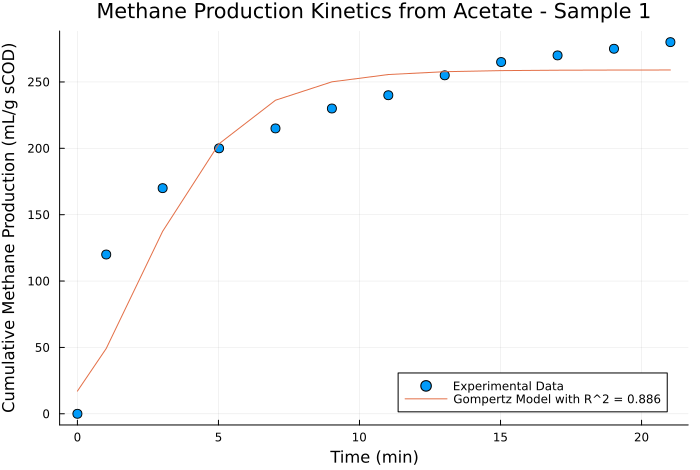
\includegraphics[width=.9\linewidth]{../plots/BMPs/Acetate/methane_kinetics_acet_test_1.png}
\end{center}

\subsection{Acetate Test 2}
\label{sec:org7aee929}
Το section αυτό αναφέρεται στη δοκιμή με 100 μL οξικό στο δείγμα (2).

\textbf{acet\textsubscript{test}\textsubscript{2}}
\begin{minted}[breaklines=true,breakanywhere=true]{julia}

### Data Analysis on Sample 2 ###

<<date_saving_acetate>>

inds = 44:57
exp_meth_vol = [0, 4, 7, 5.5, 4.5, 2.5, 2, 1, 1, 1, 0.5, 0.5, 0.45, 0.05]
exp_name = "acet_test_2"
source = "Acetate"
sample = "Sample 2"
input_cod = 0.1
p0 = [300.0, 60.0, 1.0]

<<bmp_data_processing>>
<<bmp_curve_fitting_min>>
model_acet_2 = vcat(sample, model_params, r_squared)
<<bmp_data_plotting>>
\end{minted}

\begin{table}[htbp]
\caption{Κινητικά Δεδομένα}
\centering
\begin{tabular}{lrrrr}
Timestamp & Seconds & Minutes & Methane\textsubscript{Volume} & Cumulative\textsubscript{Methane}\textsubscript{Volume}\\[0pt]
\hline
29/03\textsubscript{12}:31 & 0.0 & 0.0 & 0.0 & 0.0\\[0pt]
29/03\textsubscript{12}:32 & 25.947 & 0.4324 & 4.0 & 4.0\\[0pt]
29/03\textsubscript{12}:33 & 85.946 & 1.4324 & 7.0 & 11.0\\[0pt]
29/03\textsubscript{12}:34 & 145.935 & 2.4322 & 5.5 & 16.5\\[0pt]
29/03\textsubscript{12}:35 & 205.939 & 3.4323 & 4.5 & 21.0\\[0pt]
29/03\textsubscript{12}:36 & 265.938 & 4.4323 & 2.5 & 23.5\\[0pt]
29/03\textsubscript{12}:37 & 325.961 & 5.4327 & 2.0 & 25.5\\[0pt]
29/03\textsubscript{12}:38 & 386.204 & 6.4367 & 1.0 & 26.5\\[0pt]
29/03\textsubscript{12}:38 & 427.148 & 7.1191 & 1.0 & 27.5\\[0pt]
29/03\textsubscript{12}:39 & 487.142 & 8.1190 & 1.0 & 28.5\\[0pt]
29/03\textsubscript{12}:40 & 547.153 & 9.1192 & 0.5 & 29.0\\[0pt]
29/03\textsubscript{12}:41 & 607.15 & 10.1192 & 0.5 & 29.5\\[0pt]
29/03\textsubscript{12}:42 & 667.16 & 11.1193 & 0.45 & 29.95\\[0pt]
29/03\textsubscript{12}:43 & 722.272 & 12.0379 & 0.05 & 30.0\\[0pt]
\end{tabular}
\end{table}

\begin{center}
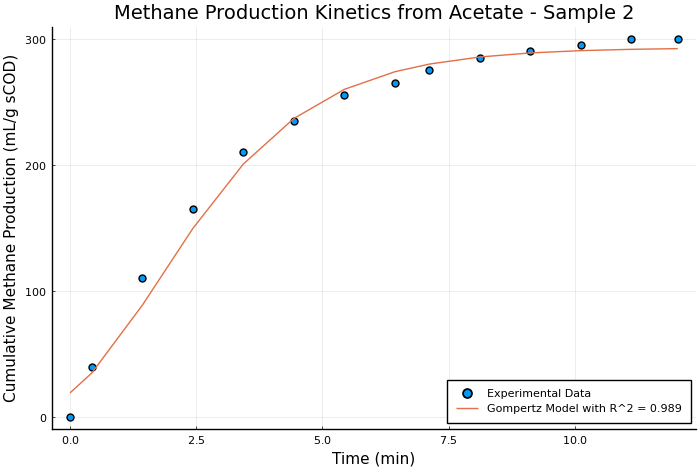
\includegraphics[width=.9\linewidth]{../plots/BMPs/Acetate/methane_kinetics_acet_test_2.png}
\end{center}

\subsection{Acetate Test 4}
\label{sec:org45d3cba}
Το section αυτό αναφέρεται στη δοκιμή με 100 μL οξικό στο δείγμα (4).

\textbf{acet\textsubscript{test}\textsubscript{4}}
\begin{minted}[breaklines=true,breakanywhere=true]{julia}

### Data Analysis on Sample 4 ###

<<date_saving_acetate>>

inds = 41:50
exp_meth_vol = [0, 4, 10, 9, 4, 5, 5, 4, 3, 3]
exp_name = "acet_test_4"
source = "Acetate"
sample = "Sample 4"
input_cod = 0.1
p0 = [400.0, 100.0, 1.0]

<<bmp_data_processing>>
<<bmp_curve_fitting_min>>
model_acet_4 = vcat(sample, model_params, r_squared)
<<bmp_data_plotting>>
\end{minted}

\begin{table}[htbp]
\caption{Κινητικά δεδομένα}
\centering
\begin{tabular}{lrrrr}
Timestamp & Seconds & Minutes & Methane\textsubscript{Volume} & Cumulative\textsubscript{Methane}\textsubscript{Volume}\\[0pt]
\hline
29/03\textsubscript{12}:29 & 0.0 & 0.0 & 0 & 0\\[0pt]
29/03\textsubscript{12}:29 & 13.397 & 0.2233 & 4 & 4\\[0pt]
29/03\textsubscript{12}:30 & 73.405 & 1.2234 & 10 & 14\\[0pt]
29/03\textsubscript{12}:31 & 133.4 & 2.2233 & 9 & 23\\[0pt]
29/03\textsubscript{12}:32 & 159.347 & 2.6558 & 4 & 27\\[0pt]
29/03\textsubscript{12}:33 & 219.346 & 3.6557 & 5 & 32\\[0pt]
29/03\textsubscript{12}:34 & 279.335 & 4.6556 & 5 & 37\\[0pt]
29/03\textsubscript{12}:35 & 339.339 & 5.6556 & 4 & 41\\[0pt]
29/03\textsubscript{12}:36 & 399.338 & 6.6556 & 3 & 44\\[0pt]
29/03\textsubscript{12}:37 & 459.361 & 7.6560 & 3 & 47\\[0pt]
\end{tabular}
\end{table}

\begin{center}
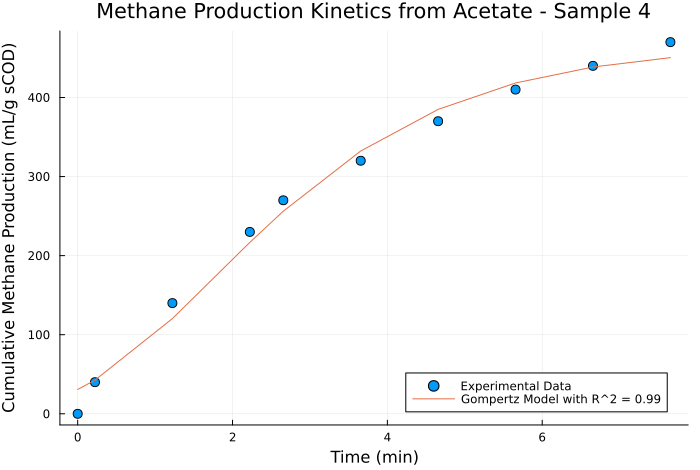
\includegraphics[width=.9\linewidth]{../plots/BMPs/Acetate/methane_kinetics_acet_test_4.png}
\end{center}

\subsection{Παραγωγή μεθανίου χωρίς feed από το δείγμα Ac}
\label{sec:org27cf0fc}
Όπως προαναφέρθηκε, το δείγμα Ac παρήγαγε μεθάνιο χωρίς να τροφοδοτηθεί με κάτι για κάποιον ανεξήγητο λόγο. Καθώς έχουμε πειραματικά δεδομένα για αυτή την κατανάλωση (και μάλιστα 2 data sets), θα γίνει και μία ανάλυση για αυτό.

\textbf{no\textsubscript{feed}\textsubscript{ac}\textsubscript{1}}
\begin{minted}[breaklines=true,breakanywhere=true]{julia}

### No Feed Data Analysis ###

<<date_saving_acetate>>

inds = 1:17
exp_meth_vol = [0, 9, 3, 2, 3, 3, 3, 2.5, 2.5, 2.5, 1.5, 3, 1, 1, 1.5, 0.5, 0.1]
exp_name = "no_feed_ac_1"
source = "No_Feed"
sample = "Sample Ac"
kinetics = false

<<bmp_data_processing>>
<<bmp_data_plotting>>
\end{minted}

\textbf{no\textsubscript{feed}\textsubscript{ac}\textsubscript{2}}
\begin{minted}[breaklines=true,breakanywhere=true]{julia}

<<date_saving_acetate>>

inds = 18:33
exp_meth_vol = [0, 3, 2, 2, 2, 3, 2, 2, 3, 2, 2.5, 2.5, 2, 2.5, 2.5, 2]
exp_name = "no_feed_ac_2"
source = "No_Feed"
sample = "Sample Ac"
kinetics = false

<<bmp_data_processing>>
<<bmp_data_plotting>>
\end{minted}

\subsection{Update all helper}
\label{sec:orgfec0fba}
Σε αυτό το section θα υπάρχει ένα helper code block που θα κάνει evaluate όλα τα παραπάνω. Έτσι, αν αλλάξει κάτι το οποίο επηρεάζει περισσότερα από ένα code blocks, θα μπορούν να γίνουν updated ταυτόχρονα πιο εύκολα. Επίσης, μία επιπλέον χρησιμότητα του code block αυτού είναι ότι αποθηκεύει ένα CSV που συγκεντρώνει όλα τα δεδομένα των κινητικών παραμέτρων από την προσαρμογή που έγινε παραπάνω, το οποίο είναι χρήσιμο για συγκρίσεις, παρόλο που τα συγκεκριμένα πειράματα δεν είναι τόσο σημαντικό να συγκριθούν.

\textbf{update\textsubscript{acetate}\textsubscript{tests}}
\begin{minted}[breaklines=true,breakanywhere=true]{julia}

<<acet_test_0>>
<<acet_test_1>>
<<acet_test_2>>
<<acet_test_4>>
<<acet_test_FW>>
<<no_feed_ac_1>>
<<no_feed_ac_2>>

model_fit_table = Tables.table(vcat(reshape(model_acet_0, 1, 5), reshape(model_acet_1, 1, 5), reshape(model_acet_2, 1, 5), reshape(model_acet_4, 1, 5), reshape(model_acet_fw, 1, 5)), header = [:Sample_Name, :Methane_Production_Potential, :Methane_Production_Rate, :Lag_Time, :R_squared])
CSV.write(datadir("exp_pro", "methane_from_acetate_kinetics.csv"), model_fit_table)
DataFrame(model_fit_table)

\end{minted}

\begin{table}[htbp]
\caption{Kinetic Models}
\centering
\begin{tabular}{lrrrr}
Sample\textsubscript{Name} & Production\textsubscript{Potential} & Production\textsubscript{Rate} & Lag\textsubscript{Time} & R\textsubscript{squared}\\[0pt]
\hline
Sample 0 & 452.518 & 80.388 & 0.0 & 0.967\\[0pt]
Sample 1 & 208.238 & 55.028 & 0.0 & 0.960\\[0pt]
Sample 2 & 292.865 & 61.914 & 0.0 & 0.989\\[0pt]
Sample 4 & 466.239 & 97.778 & 0.0 & 0.990\\[0pt]
Sample FW & 255.214 & 55.941 & 0.0 & 0.896\\[0pt]
\end{tabular}
\end{table}

\subsection{Γενικά σχόλια για αυτόν τον κύκλο πειραμάτων}
\label{sec:orge5d4edc}
Ο πρώτος αυτός κύκλος πειραμάτων ήταν για την δοκιμή προσθήκης οξικού οξέος, του ιδανικού υποστρώματος της μεθανογένεσης, για να δούμε πως θα αντιδράσει σε αυτό το σύστημα. Δεν έχει τόσο συγκριτικό χαρακτήρα μεταξύ των πειραμάτων (παρόλο που ένα σχόλιο που μπορεί να γίνει είναι πως τα πειράματα τα οποία ήταν ίδια πρακτικά στην αρχή, είχαν αρκετά διαφορετική απόκριση στην προσθήκη οξικού), αλλά τον χαρακτήρα της βέλτιστης δυνατής μεθανογένεσης από κάποιο υπόστρωμα. Από την μελέτη αυτή, προέκυψαν αρκετά συμπεράσματα.

Ένα ενδιαφέρον σχόλιο είναι πως το σύστημα ανταποκρίνεται στην προσθήκη του οξικού πολύ γρήγορα (μετά από μερικά δευτερόλεπτα κιόλας βλέπουμε παραγωγή μεθανίου) και στο μοντέλο αυτό μεταφράζεται ως μηδενικό lag-phase.

Το δείγμα 4 είχε αναπάντεχα υψηλό ρυθμό παραγωγής μεθανίου, το οποίο φάνηκε από το γεγονός ότι παράχθηκε την μέγιστη ποσότητα οξικού που περιμέναμε σε περίπου 7 λεπτά ενώ τα υπόλοιπα χρειάστηκαν τουλάχιστον 15 λεπτά. Αυτό φάνηκε και στο μοντέλο, όπου το δείγμα αυτό είχε πολύ υψηλό ειδικό ρυθμό παραγωγής μεθανίου. Το δείγμα Ac ήταν αυτό που παρήγαγε αέριο χωρίς κάποιο υπόστρωμα. Μόλις προστέθηκε οξικό, αντέδρασε σε αυτό και ο ρυθμός του αυξήθηκε, αλλά επιβράδυνε πολύ γρήγορα, με αποτέλεσμα να έχει πολύ αργό ρυθμό παραγωγής μεθανίο και το χαμηλότερο δυναμικό παραγωγής μεθανίου. Μπορεί η αλλαγή αυτή να ευθύνεται σε αυτήν την απόκριση. Τα δείγματα 0 και 4 είχαν πολύ μεγαλύτερη παραγωγικότητα από τα άλλα 3, χωρίς να υπάρχει κάποια εύκολη εξήγηση για αυτό.

\pagebreak

\section{FW Hydrolysate 1 Processing}
\label{sec:org9828d9f}
Στο section αυτό θα αναλυθούν τα αποτελεσματα του πρώτου πειράματος που χρησιμοποιήσε FW hydrolysate ως υπόστρωμα. Σκοπός είναι να γίνει μία σύγκριση αυτού με το οξικό για κάθε δοχείο για να προκύψουν αποτελέσματα για το κάθε πείραμα. Οι 5 δοκιμές που έγιναν ήταν στα δείγματα 0, 1, 2 και 4 (τα οποία πλέον έχουν νόημα επειδή εκφράζουν την ποσότητα mix που προστέθηκε κατά την υδρόλυση) αλλά επίσης έγινε και ένα πείραμα για να μετρηθεί η απόδοση σε μεθάνιο του δείγματος μόνο με FW (ενδέχεται να υπήρξε διαρροή στο δείγμα αυτό καθώς η παραγωγή ήταν απειροελάχιστη).

\subsection{Sample 0}
\label{sec:org5c92806}
Το δείγμα αυτό είναι labelled ως δείγμα 0 καθώς είναι το δείγμα το οποίο τροφοδοτήθηκε με treated FW, όμως χωρίς προσθήκη του μιξ ενζύμων και μικροοργανισμών. Όπως έχουμε δεί, όλες οι αντιδράσεις που γίνονται κατά την υδρόλυση και ζύμωση μπορούν να γίνουν και χωρίς το μιξ. Όμως, γινόντουσαν πιο αποτελεσματικά με την προσθήκη αυτού. Οπότε, ελπίζουμε πως το δείγμα αυτό θα έχει χειρότερα αποτελέσματα από τα άλλα, το οποίο θα μας οδηγήσει στην υπόθεση ότι το μιξ βελτιώνει όχι μόνο τα κριτήρια υδρόλυσης και οξεογένεσης αλλά και αυτό της μεθανογένεσης.

\textbf{hydrolysate\textsubscript{0}\textsubscript{ad}}
\begin{minted}[breaklines=true,breakanywhere=true]{julia}

### Data Analysis on Hydrolysate with 0 ml ###

<<date_saving_fw_1>>

inds = 1:34
exp_meth_vol = [0, 1.0, 0.2, 0.02, 0.02, 0.01, 0.2, 0.2, 0.5, 0.2, 0.5, 1.5, 0.05, 0.05, 0.05, 0.05, 0.05, 0.05, 0.1, 0.1, 0.1, 0.1, 0.1, 0.1, 0.1, 0.1, 0.1, 0.1, 0.1, 0.1, 0.1, 0.05, 0.05, 0.05]

exp_name = "hydrolysate_0"
source = "Hydrolyzed FW"
sample = "Sample 0"
input_cod = 0.1

<<bmp_data_processing>>

# The same model is fit either with min or hour
p0 = [50.0, 0.4, 1.0]
<<bmp_curve_fitting_min>>
model_hydro_0_min = vcat(sample, model_params, r_squared)
<<bmp_data_plotting>>

p0 = [40.0, 1.0, 1.0]
<<bmp_curve_fitting_hour>>
model_hydro_0_hour = vcat(sample, model_params, r_squared)
<<bmp_data_plotting>>
\end{minted}

\subsubsection{Results}
\label{sec:org14bddc7}
Παρακάτω φαίνονται τα αποτελέσματα του σχετικού πειράματος.

Παρήγαγε 6.1 ml μεθανίου, το οποίο είναι το \(12.8 \%\) του πειράματος με οξικό. Σχετικά με την προσαρμογή των δεδομένων του σε ένα μοντέλο Gompertz, υπάρχουν 2 πιθανά μοντέλα που ταιριάζουν στο πείραμα. Στο πρώτο, ο ειδικός ρυθμός ανάπτυξης είναι μεγάλος, το οποίο κάνει fit τέλεια στις μετρήσεις της πρώτης ώρας όπου η παραγωγή είναι γρήγορη. Όμως, προβλέπει την στάσιμη φάση λίγες ώρες μετά, το οποίο δεν ισχύει καθώς την 2η μέρα υπάρχει μία καλή παραγωγικότητα μεθανίου. Παρόλα αυτά, έχει καλό R\textsuperscript{2}. Αυτό το μοντέλο είναι πιο εύκολο να προβλεφθεί με x άξονα σε λεπτά, όπου δεν χρειάζεται πάρα πολύ υψηλή αρχική συνθήκη. Ο προβλεπόμενος ειδικός ρυθμός ανάπτυξης θα είναι \(0.384 \frac{ml}{g ~ sCOD \min } \text{ ή } 23.03 \frac{ml}{g ~ sCOD hour}\).

Όμως, υπάρχει και ένα δεύτερο μοντέλο με καλή προσαρμογή (μάλιστα είναι ελαφρώς καλύτερη). Αν ο ειδικός ρυθμός ανάπτυξης είναι χαμηλός, υπάρχει μοντέλο που προσαρμόζεται σχεδόν τέλεια στην 2η και 3η μέρα. Συγκεκριμένα, με ειδικό ρυθμό \(1.636 \frac{ml}{g ~ sCOD ~ hour}\) πετυχαίνεται μία πολύ καλή προσαρμογή. Όμως, αυτό είναι αρκετά λάθος για την πρώτη μέρα.

Ένα πιθανό συμπέρασμα μπορεί να είναι πως κάτι συμβαίνει στον αντιδραστήρα το οποίο επιβραδύνει σημαντικά τον μέγιστο ειδικό ρυθμό ανάπτυξης, ο οποίος μπαίνει στο μοντέλο.

\begin{center}
\begin{tabular}{lrrrr}
Timestamp & Minutes & Hours & Methane\textsubscript{Volume} & Cumulative\textsubscript{Methane}\textsubscript{Volume}\\[0pt]
\hline
01/04\textsubscript{11}:05 & 0.0 & 0.0 & 0.0 & 0.0\\[0pt]
01/04\textsubscript{11}:09 & 3.7328 & 0.0622 & 1.0 & 1.0\\[0pt]
01/04\textsubscript{11}:11 & 5.733 & 0.0956 & 0.2 & 1.2\\[0pt]
01/04\textsubscript{11}:12 & 6.7332 & 0.1122 & 0.02 & 1.22\\[0pt]
01/04\textsubscript{11}:13 & 7.5618 & 0.126 & 0.02 & 1.24\\[0pt]
01/04\textsubscript{11}:14 & 8.5617 & 0.1427 & 0.01 & 1.25\\[0pt]
01/04\textsubscript{11}:15 & 9.5618 & 0.1594 & 0.2 & 1.45\\[0pt]
01/04\textsubscript{11}:21 & 16.0005 & 0.2667 & 0.2 & 1.65\\[0pt]
01/04\textsubscript{11}:52 & 46.3266 & 0.7721 & 0.5 & 2.15\\[0pt]
01/04\textsubscript{12}:22 & 76.3266 & 1.2721 & 0.2 & 2.35\\[0pt]
01/04\textsubscript{16}:52 & 346.3272 & 5.7721 & 0.5 & 2.85\\[0pt]
02/04\textsubscript{10}:54 & 1428.1379 & 23.8023 & 1.5 & 4.35\\[0pt]
02/04\textsubscript{12}:54 & 1548.1453 & 25.8024 & 0.05 & 4.4\\[0pt]
02/04\textsubscript{13}:24 & 1578.1452 & 26.3024 & 0.05 & 4.45\\[0pt]
02/04\textsubscript{13}:54 & 1608.1455 & 26.8024 & 0.05 & 4.5\\[0pt]
02/04\textsubscript{14}:24 & 1638.1455 & 27.3024 & 0.05 & 4.55\\[0pt]
02/04\textsubscript{14}:54 & 1668.1454 & 27.8024 & 0.05 & 4.6\\[0pt]
02/04\textsubscript{15}:24 & 1698.1453 & 28.3024 & 0.05 & 4.65\\[0pt]
02/04\textsubscript{15}:54 & 1728.1453 & 28.8024 & 0.1 & 4.75\\[0pt]
02/04\textsubscript{16}:24 & 1758.1455 & 29.3024 & 0.1 & 4.85\\[0pt]
02/04\textsubscript{16}:54 & 1788.1455 & 29.8024 & 0.1 & 4.95\\[0pt]
02/04\textsubscript{17}:24 & 1818.1452 & 30.3024 & 0.1 & 5.05\\[0pt]
02/04\textsubscript{17}:54 & 1848.152 & 30.8025 & 0.1 & 5.15\\[0pt]
02/04\textsubscript{19}:54 & 1968.1526 & 32.8025 & 0.1 & 5.25\\[0pt]
02/04\textsubscript{21}:54 & 2088.1542 & 34.8026 & 0.1 & 5.35\\[0pt]
02/04\textsubscript{23}:54 & 2208.1584 & 36.8026 & 0.1 & 5.45\\[0pt]
03/04\textsubscript{01}:54 & 2328.1584 & 38.8026 & 0.1 & 5.55\\[0pt]
03/04\textsubscript{03}:54 & 2448.1582 & 40.8026 & 0.1 & 5.65\\[0pt]
03/04\textsubscript{05}:54 & 2568.1632 & 42.8027 & 0.1 & 5.75\\[0pt]
03/04\textsubscript{07}:54 & 2688.1651 & 44.8028 & 0.1 & 5.85\\[0pt]
03/04\textsubscript{09}:54 & 2808.1652 & 46.8028 & 0.1 & 5.95\\[0pt]
03/04\textsubscript{12}:54 & 2988.1741 & 49.8029 & 0.05 & 6.0\\[0pt]
03/04\textsubscript{13}:54 & 3048.1739 & 50.8029 & 0.05 & 6.05\\[0pt]
03/04\textsubscript{14}:24 & 3078.1749 & 51.3029 & 0.05 & 6.1\\[0pt]
\end{tabular}
\end{center}

\begin{center}
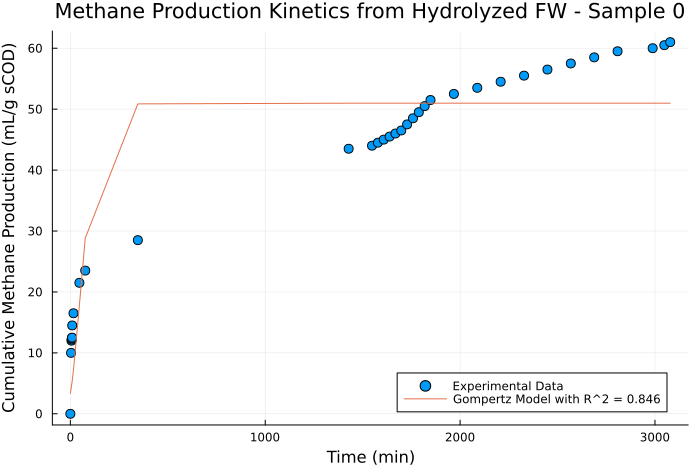
\includegraphics[width=.9\linewidth]{../plots/BMPs/Hydrolyzed FW/methane_kinetics_hydrolysate_0_min.png}
\end{center}

\begin{center}
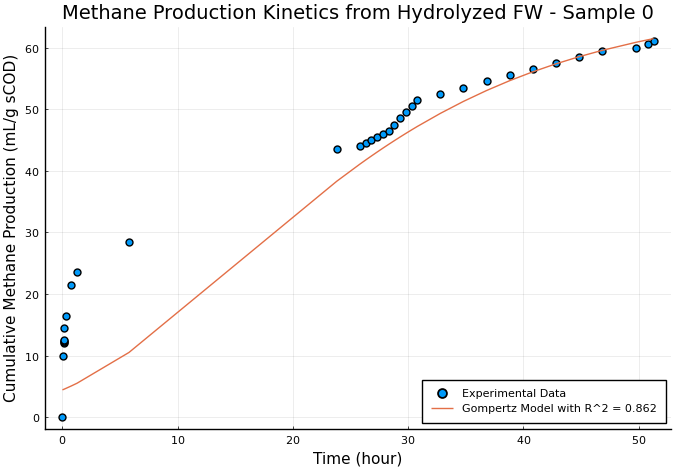
\includegraphics[width=.9\linewidth]{../plots/BMPs/Hydrolyzed FW/methane_kinetics_hydrolysate_0_hour.png}
\end{center}

\subsection{Sample 1}
\label{sec:org8133c1c}
Το δείγμα αυτό τροφοδοτήθηκε με το υδρόλυμα το οποίο είχε προσθήκη 1 ml mix. Στο αρχικό κινητικό πείραμα, το δείγμα αυτό είχε αρκετά παρόμοια συμπεριφορά με το 0 και χειρότερη αυτής του 1. Από την μέτρηση του COD του, είχε αναπάντεχα υψηλό sCOD. Αυτό σημαίνει είτε πως έγινε κάποιο λάθος στην ανάλυση ή ότι απλώς έγινε πολύ καλύτερη υδρόλυση από ότι περιμέναμε στο πείραμα αυτό. Με βάση το sCOD του, αναμένεται να έχει καλά αποτελέσματα. Με βάση την HPLC του αρχικού πειράματος, θα περιμέναμε να είναι λίγο καλύτερο από το 0.

\textbf{hydrolysate\textsubscript{1}\textsubscript{ad}}
\begin{minted}[breaklines=true,breakanywhere=true]{julia}

### Data Analysis on Hydrolysate with 1 ml ###

<<date_saving_fw_1>>

inds = 2:34
exp_meth_vol = [0, 2.0, 0.5, 0.5, 0.5, 0.5, 0.5, 0, 0.2, 0.5, 2.0, 0.3, 0.3, 0.3, 0.1, 0.6, 0.6, 0.5, 0.5, 0.5, 0.4, 0.6, 0.1, 0.05, 0.05, 0.05, 0.05, 0.05, 0.05, 0.05, 0.3, 0.2, 0.2]
exp_name = "hydrolysate_1"
source = "Hydrolyzed FW"
sample = "Sample 1"
input_cod = 0.1

p0 = [130.0, 10.0, 1.0]
<<bmp_data_processing>>
<<bmp_curve_fitting_min>>
model_hydro_1_min = vcat(sample, model_params, r_squared)
<<bmp_data_plotting>>

p0 = [200.0, 5.0, 1.0]
<<bmp_curve_fitting_hour>>
model_hydro_1_hour = vcat(sample, model_params, r_squared)
<<bmp_data_plotting>>
\end{minted}

\subsubsection{Results}
\label{sec:org6171be6}
Το πείραμα αυτό παρήγαγε 13.05 ml μεθάνιο, το οποίο είναι το \(60.7 \%\) του πειράματος με οξικό καθώς εκείνο το πείραμα είχε μία σχετικά χαμηλή παραγωγικότητα για οξικό. Υπάρχει η σκέψη ότι μπορεί λόγω της διεργασίας που συνέβαινε αρχικά στο δείγμα αυτό (παραγωγή μεθανίου χωρίς τροφή) να επηρεάστηκε η παραγωγικότητα του και αυτό το ποσοστό να μην είναι τόσο έμπιστο.

Από άποψη προσαρμογής, το πείραμα αυτό έχει το πρόβλημα πως μεταξύ της 2ης και 3ης μέρας όχι μόνο επιβραδύνθηκε αρκετά το πείραμα (όπως στο 0 ml) αλλά σχεδόν σταμάτησε. Όμως, το πρωί της τρίτης μέρας, λίγο πριν σταματήσουμε το πείραμα, η παραγωγή αυξήθηκε σχετικά σημαντικά. Οπότε, η προσαρμογή του είναι λίγο πιο δύσκολη. Υπάρχει πάλι το φαινόμενο των 2 ρυθμών (ενός γρήγορου για τα δείγματα της 1ης μέρας και ενός αργού για μετά), όμως, ο γρήγορος είναι σημαντικά χειρότερος εδώ (R\textsuperscript{2} 0.689 αντί για 0.815), προβλέπει με λιγότερη ακρίβεια ακόμη και την πρώτη μέρα και η στάσιμη φάση του είναι πολύ χαμηλά. Ο αργός ρυθμός είναι και αυτός σχετικά λάθος επειδή δεν μπορεί να προβλέψει την δημιουργία στάσιμης φάσης και μετά επανεκίννησης της χώνευσης (κάτι που δεν νομίζω να προβλέπεται από οποιοδήποτε μοντέλο). Οπότε, κάνει underestimate το σημείο που ακόμη παράγει και overestimate όταν έχει αρχίσει η στάσιμη φάση. Βέβαια, για τόσα πειραματικά σημεία (τα οποία έχουν και κάποια προβλήματα που δεν μπορούν να εξηγηθούν εύκολα), η προσαρμογή με R\textsuperscript{2} = 0.815 είναι σχετικά καλή.

Το μοντέλο με τον γρήγορο ρυθμό έχει ειδικό ρυθμό ανάπτυξης \(0.841 \frac{ml}{g ~ sCOD min } \text{ ή } 50.43 \frac{ml}{g ~ sCOD hour}\) ενώ το αργό έχει ρυθμό \(3.175 \frac{ml}{g ~ sCOD hour}\).

\begin{center}
\begin{tabular}{lrrrr}
Timestamp & Minutes & Hours & Methane\textsubscript{Volume} & Cumulative\textsubscript{Methane}\textsubscript{Volume}\\[0pt]
\hline
01/04\textsubscript{11}:09 & 0.0 & 0.0 & 0.0 & 0.0\\[0pt]
01/04\textsubscript{11}:11 & 2.0003 & 0.0333 & 2.0 & 2.0\\[0pt]
01/04\textsubscript{11}:12 & 3.0004 & 0.05 & 0.5 & 2.5\\[0pt]
01/04\textsubscript{11}:13 & 3.829 & 0.0638 & 0.5 & 3.0\\[0pt]
01/04\textsubscript{11}:14 & 4.8289 & 0.0805 & 0.5 & 3.5\\[0pt]
01/04\textsubscript{11}:15 & 5.8291 & 0.0972 & 0.5 & 4.0\\[0pt]
01/04\textsubscript{11}:21 & 12.2677 & 0.2045 & 0.5 & 4.5\\[0pt]
01/04\textsubscript{11}:52 & 42.5938 & 0.7099 & 0.0 & 4.5\\[0pt]
01/04\textsubscript{12}:22 & 72.5938 & 1.2099 & 0.2 & 4.7\\[0pt]
01/04\textsubscript{16}:52 & 342.5944 & 5.7099 & 0.5 & 5.2\\[0pt]
02/04\textsubscript{10}:54 & 1424.4052 & 23.7401 & 2.0 & 7.2\\[0pt]
02/04\textsubscript{12}:54 & 1544.4126 & 25.7402 & 0.3 & 7.5\\[0pt]
02/04\textsubscript{13}:24 & 1574.4125 & 26.2402 & 0.3 & 7.8\\[0pt]
02/04\textsubscript{13}:54 & 1604.4127 & 26.7402 & 0.3 & 8.1\\[0pt]
02/04\textsubscript{14}:24 & 1634.4127 & 27.2402 & 0.1 & 8.2\\[0pt]
02/04\textsubscript{14}:54 & 1664.4126 & 27.7402 & 0.6 & 8.8\\[0pt]
02/04\textsubscript{15}:24 & 1694.4125 & 28.2402 & 0.6 & 9.4\\[0pt]
02/04\textsubscript{15}:54 & 1724.4125 & 28.7402 & 0.5 & 9.9\\[0pt]
02/04\textsubscript{16}:24 & 1754.4128 & 29.2402 & 0.5 & 10.4\\[0pt]
02/04\textsubscript{16}:54 & 1784.4128 & 29.7402 & 0.5 & 10.9\\[0pt]
02/04\textsubscript{17}:24 & 1814.4125 & 30.2402 & 0.4 & 11.3\\[0pt]
02/04\textsubscript{17}:54 & 1844.4193 & 30.7403 & 0.6 & 11.9\\[0pt]
02/04\textsubscript{19}:54 & 1964.4198 & 32.7403 & 0.1 & 12.0\\[0pt]
02/04\textsubscript{21}:54 & 2084.4214 & 34.7404 & 0.05 & 12.05\\[0pt]
02/04\textsubscript{23}:54 & 2204.4256 & 36.7404 & 0.05 & 12.1\\[0pt]
03/04\textsubscript{01}:54 & 2324.4257 & 38.7404 & 0.05 & 12.15\\[0pt]
03/04\textsubscript{03}:54 & 2444.4255 & 40.7404 & 0.05 & 12.2\\[0pt]
03/04\textsubscript{05}:54 & 2564.4305 & 42.7405 & 0.05 & 12.25\\[0pt]
03/04\textsubscript{07}:54 & 2684.4324 & 44.7405 & 0.05 & 12.3\\[0pt]
03/04\textsubscript{09}:54 & 2804.4325 & 46.7405 & 0.05 & 12.35\\[0pt]
03/04\textsubscript{12}:54 & 2984.4414 & 49.7407 & 0.3 & 12.65\\[0pt]
03/04\textsubscript{13}:54 & 3044.4412 & 50.7407 & 0.2 & 12.85\\[0pt]
03/04\textsubscript{14}:24 & 3074.4422 & 51.2407 & 0.2 & 13.05\\[0pt]
\end{tabular}
\end{center}

\begin{center}
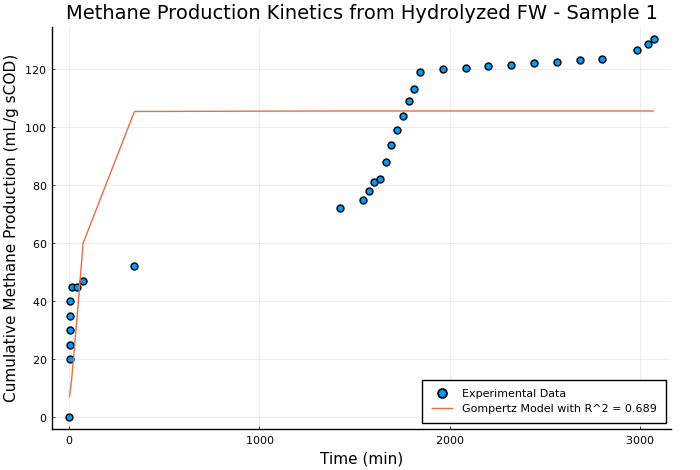
\includegraphics[width=.9\linewidth]{../plots/BMPs/Hydrolyzed FW/methane_kinetics_hydrolysate_1_min.png}
\end{center}

\begin{center}
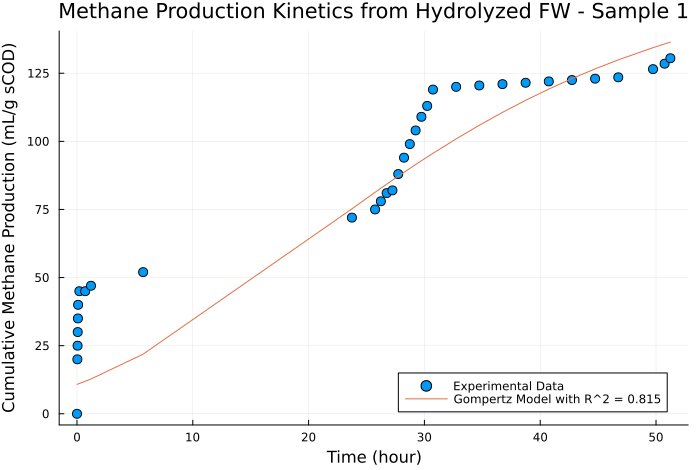
\includegraphics[width=.9\linewidth]{../plots/BMPs/Hydrolyzed FW/methane_kinetics_hydrolysate_1_hour.png}
\end{center}

\subsection{Sample 2}
\label{sec:org9f206ab}
Το δείγμα το οποίο στην υδρόλυση είχε 2 ml από το μιξ. Με βάση το αρχικό πείραμα υδρόλυσης, αυτό και το 4 ml είχαν το καλύτερο performance και ελάχιστη διαφορά μεταξύ τους (κατά βάση στην συγκέντρωση γαλακτικού οξέος) οπότε θα αναμέναμε εδώ να παρατηρηθεί η καλύτερη μεθανογένεση.

\textbf{hydrolysate\textsubscript{2}\textsubscript{ad}}
\begin{minted}[breaklines=true,breakanywhere=true]{julia}

### Data Analysis on Hydrolysate with 2 ml ###

<<date_saving_fw_1>>

inds = 7:34
exp_meth_vol = [0, 6, 0.5, 0.1, 0.5, 1.5, 0.2, 0.1, 0.1, 0.1, 0.1, 0.1, 0.1, 0.1, 0.1, 0.1, 0.1, 0.1, 0.1, 0.1, 0.1, 0.1, 0.1, 0.1, 0.1, 0.1, 0.2, 0.2]
exp_name = "hydrolysate_2"
source = "Hydrolyzed FW"
sample = "Sample 2"
input_cod = 0.1

<<bmp_data_processing>>

p0 = [100.0, 15.0, 1.0]
<<bmp_curve_fitting_min>>
model_hydro_2_min = vcat(sample, model_params, r_squared)
<<bmp_data_plotting>>

p0 = [100.0, 1.0, 0.03]
<<bmp_curve_fitting_hour>>
model_hydro_2_hour = vcat(sample, model_params, r_squared)
<<bmp_data_plotting>>
\end{minted}

\subsubsection{Results}
\label{sec:orga46991a}
Το παραγώμενο μεθάνιο είναι 11.1 ml, δηλαδή \(37 \%\) του προβλεπόμενου μεθανίου με βάση το οξικό.

Ένα πολύ βασικό πρόβλημα του πειράματος αυτού είναι πως έχουμε μία μεγάλη παραγωγικότητα μεθανίου στην πρώτη φωτογραφία, όμως αυτή ήταν 6.5 λεπτά μετά την αρχή. Οπότε, δύνανται να υπάρχουν πάρα πολλά κινητικά μοντέλα τα οποία είναι αποδεχτά. Αξίζει να σημειωθεί πως το καλύτερο R\textsuperscript{2} είναι 0.724, το οποίο δείχνει πως κανένα από τα μοντέλα δεν είναι ιδιαίτερα αξιόπιστο. Το πρόβλημα της δειγματοληψίας αυτής είναι πιθανόν να φταίει.

Τα τέσσερα δυνατά μοντέλα διακρίνονται ως εξής: Μπορεί ο ρυθμός να είναι αρκετά χαμηλός ώστε να προσωμοιώνει το τέλος της χώνευσης, το οποίο είναι αργό. Ο ρυθμός αυτός είναι \(0.031 \frac{ml}{g ~ sCOD \min } \text{ ή } 1.88 \frac{ml}{g ~ sCOD \min }\), ο οποίος είναι παρόμοιας τάξης μεγέθους με τον αργό ρυθμό των άλλων δειγμάτων. Όπως και στο sample 1 όμως, το αποτέλεσμα αυτό δεν έχει καλό R\textsuperscript{2} και μάλλον δεν θεωρείται έμπιστο. Το άλλο μοντέλο που ακολουθεί την λογική των παραπάνω είναι το χειρότερο δυνατό μοντέλο (R\textsuperscript{2} = 0.639) το οποίο έχει ειδικό ρυθμό ανάπτυξης \(1.192 \frac{ml}{g ~ sCOD \min }\) (ο οποίος είναι παρόμοιας τάξης μεγέθους με τους άλλους 2, αλλά λίγο μεγαλύτερος) και την λογική ότι στα πρώτα 6 λεπτά παράχθηκε το περισσότερο μεθάνιο. Το καλύτερο δυνατό μοντέλο έχει παρόμοια λογική πολύ γρήγορου ειδικού ρυθμού ανάπτυξης \(\left( 15.483 \frac{ml}{g ~ sCOD \min } \right)\), αλλά ένα lag phase 2.42 λεπτών. Η λογική που μπορούν να ισχύουν και τα δύο είναι ότι βλέπουμε αποτέλεσμα σε 6.5 λεπτά περίπου, οπότε, μπορεί να υπήρχε ένα lag time στην αρχή και μετά να εξελίχθηκε πιο γρήγορα το φαινόμενο. Επίσης, ένα μοντέλο με ακόμη μεγαλύτερο lag time αλλά και ειδικό ρυθμό ανάπτυξης προέκυψε και είχε σχεδόν identical R\textsuperscript{2} με το παραπάνω. Καθώς κανένα άλλο μοντέλο δεν έχει παρουσιάσει lag time, το πιο εύλογο θα ήταν να ισχύει ένα από τα 2 πρώτα μοντέλα. Όμως, απουσία άλλων δεδομένων, το καλύτερο μοντέλο είναι αυτό με το μικρό lag phase.

\begin{center}
\begin{tabular}{lrrrr}
Timestamp & Minutes & Hours & Methane\textsubscript{Volume} & Cumulative\textsubscript{Methane}\textsubscript{Volume}\\[0pt]
\hline
01/04\textsubscript{11}:15 & 0.0 & 0.0 & 0.0 & 0.0\\[0pt]
01/04\textsubscript{11}:21 & 6.4386 & 0.1073 & 6.0 & 6.0\\[0pt]
01/04\textsubscript{11}:52 & 36.7648 & 0.6127 & 0.5 & 6.5\\[0pt]
01/04\textsubscript{12}:22 & 66.7647 & 1.1127 & 0.1 & 6.6\\[0pt]
01/04\textsubscript{16}:52 & 336.7653 & 5.6128 & 0.5 & 7.1\\[0pt]
02/04\textsubscript{10}:54 & 1418.5761 & 23.6429 & 1.5 & 8.6\\[0pt]
02/04\textsubscript{12}:54 & 1538.5835 & 25.6431 & 0.2 & 8.8\\[0pt]
02/04\textsubscript{13}:24 & 1568.5834 & 26.1431 & 0.1 & 8.9\\[0pt]
02/04\textsubscript{13}:54 & 1598.5836 & 26.6431 & 0.1 & 9.0\\[0pt]
02/04\textsubscript{14}:24 & 1628.5836 & 27.1431 & 0.1 & 9.1\\[0pt]
02/04\textsubscript{14}:54 & 1658.5836 & 27.6431 & 0.1 & 9.2\\[0pt]
02/04\textsubscript{15}:24 & 1688.5834 & 28.1431 & 0.1 & 9.3\\[0pt]
02/04\textsubscript{15}:54 & 1718.5834 & 28.6431 & 0.1 & 9.4\\[0pt]
02/04\textsubscript{16}:24 & 1748.5837 & 29.1431 & 0.1 & 9.5\\[0pt]
02/04\textsubscript{16}:54 & 1778.5837 & 29.6431 & 0.1 & 9.6\\[0pt]
02/04\textsubscript{17}:24 & 1808.5834 & 30.1431 & 0.1 & 9.7\\[0pt]
02/04\textsubscript{17}:54 & 1838.5902 & 30.6432 & 0.1 & 9.8\\[0pt]
02/04\textsubscript{19}:54 & 1958.5907 & 32.6432 & 0.1 & 9.9\\[0pt]
02/04\textsubscript{21}:54 & 2078.5923 & 34.6432 & 0.1 & 10.0\\[0pt]
02/04\textsubscript{23}:54 & 2198.5966 & 36.6433 & 0.1 & 10.1\\[0pt]
03/04\textsubscript{01}:54 & 2318.5966 & 38.6433 & 0.1 & 10.2\\[0pt]
03/04\textsubscript{03}:54 & 2438.5964 & 40.6433 & 0.1 & 10.3\\[0pt]
03/04\textsubscript{05}:54 & 2558.6014 & 42.6434 & 0.1 & 10.4\\[0pt]
03/04\textsubscript{07}:54 & 2678.6033 & 44.6434 & 0.1 & 10.5\\[0pt]
03/04\textsubscript{09}:54 & 2798.6034 & 46.6434 & 0.1 & 10.6\\[0pt]
03/04\textsubscript{12}:54 & 2978.6123 & 49.6435 & 0.1 & 10.7\\[0pt]
03/04\textsubscript{13}:54 & 3038.6121 & 50.6435 & 0.2 & 10.9\\[0pt]
03/04\textsubscript{14}:24 & 3068.6131 & 51.1436 & 0.2 & 11.1\\[0pt]
\end{tabular}
\end{center}

\begin{center}
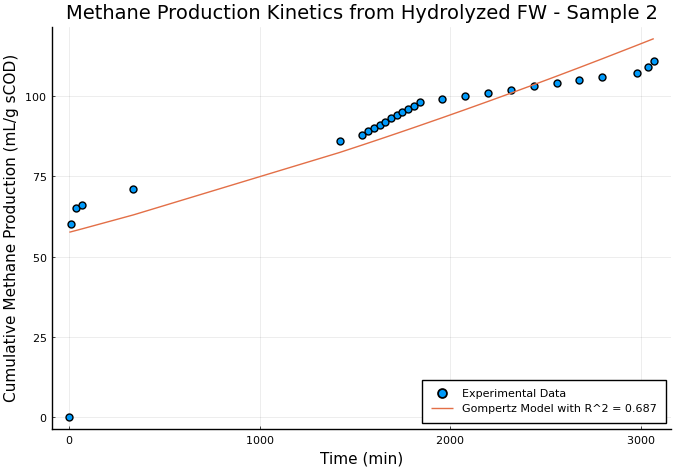
\includegraphics[width=.9\linewidth]{../plots/BMPs/Hydrolyzed FW/methane_kinetics_hydrolysate_2_min.png}
\end{center}

\begin{center}
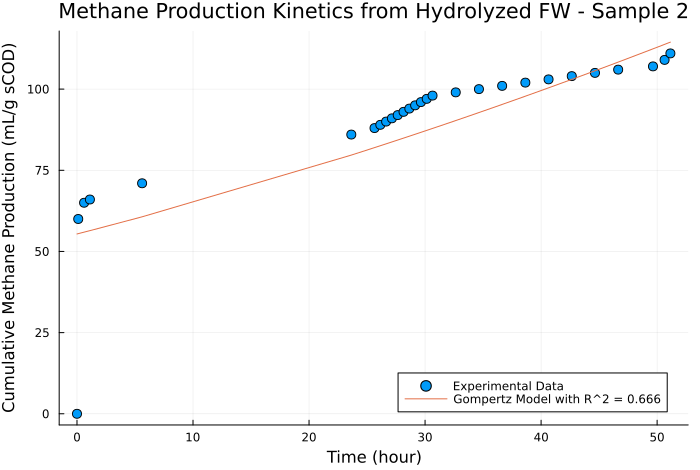
\includegraphics[width=.9\linewidth]{../plots/BMPs/Hydrolyzed FW/methane_kinetics_hydrolysate_2_hour.png}
\end{center}

\subsection{Sample 4}
\label{sec:orgb4d477d}
Το δείγμα 4 ήταν αυτό με τα 4 ml mix στην υδρόλυση. Είναι η μέγιστη ποσότητα που χρησιμοποιήθηκε για τα πειράματα χώνευσης καθώς το 8 ml δεν είχε ιδιαίτερα μεγάλη διαφορά και είναι πολύ πιο ακριβό. Όπως προαναφέρθηκε, αναμένουμε να έχει παρόμοια ποιότητα με το 2 ml καθώς με εξαίρεση μίας ποσότητας γαλακτικού είναι σχεδόν ίδια.

\textbf{hydrolysate\textsubscript{4}\textsubscript{ad}}
\begin{minted}[breaklines=true,breakanywhere=true]{julia}

### Data Analysis on Hydrolysate with 4 ml ###

<<date_saving_fw_1>>

inds = 5:34
exp_meth_vol = [0, 13, 0.1, 0.2, 0.1, 0.2, 0.5, 1, 0.4, 0.1, 0.3, 0.1, 0.1, 0.1, 0.0, 0.0, 0.0, 0.05, 0.05, 0.05, 0.05, 0.05, 0.05, 0.05, 0.05, 0.05, 0.2, 0.2, 0.2, 0.1]
exp_name = "hydrolysate_4"
source = "Hydrolyzed FW"
sample = "Sample 4"
input_cod = 0.1

<<bmp_data_processing>>

p0 = [170.0, 150.0, 1.0]
<<bmp_curve_fitting_min>>
model_hydro_4_min = vcat(sample, model_params, r_squared)
<<bmp_data_plotting>>

p0 = [170.0, 1000.0, 0.1]
<<bmp_curve_fitting_hour>>
model_hydro_4_hour = vcat(sample, model_params, r_squared)
<<bmp_data_plotting>>
\end{minted}

\subsubsection{Results}
\label{sec:orgf3350d1}
Το δείγμα αυτό είχε την ιδιαιτερότητα της μεγαλύτερης παραγωγής μεθανίου από όλα τα δείγματα σε αρκετά γρήγορο ρυθμό, κάτι που προβλέπεται καθώς ήταν και η συμπεριφορά της λάσπης του. Η παραγωγή 17.35 ml μεθανίου είναι το \(36.9 \%\) αυτής του οξικού οξέος. Το γεγονός ότι είναι το ίδιο ποσοστό με αυτό του 2 ml είναι αρκετά καλό.

Επίσης, η παραγωγή είναι περίεργη καθώς παράγονται 13 ml μέσα σε ένα λεπτό και μετά το σύστημα μπαίνει σε μία σχεδόν στάσιμη φάση όπου η παραγωγή μεθανίου έχει επιβραδυνθεί σημαντικά, αλλά συνεχίζει να παράγει κάποια μικρή ποσότητα μέχρι και τις 51 ώρες όπου σταμάτησε το πείραμα. Οπότε, το γεγονός ότι το μοντέλο που προβλέπεται είναι ένα με πάρα πολύ υψηλό ειδικό ρυθμό ανάπτυξης το οποίο φτάνει σε στάσιμη φάση στα πρώτα λεπτά είναι αναμενόμενο.

Όμως, σε αντίθεση με τα άλλα πειράματα, αυτό είναι σχεδόν ολόσωστο σαν ιδέα καθώς 51 ώρες δεν παρήγαγαν ούτε το μισό του πρώτου λεπτού, οπότε παρόλο που θα αναμέναμε λίγο περισσότερη καμπύλη και όχι την μορφη που προκύπτει (η οποία είναι ουσιαστικά μία κατακόρυφη και μία οριζόντια γραμμή), η εξίσωση αυτή προβλέπει σχετικά καλά την πραγματικότητα και το R\textsuperscript{2} είναι 0.865, το οποίο είναι η καλύτερη προσαρμογή που έχουμε δεί σε ένα από αυτά τα πειράματα. Ο ειδικός ρυθμός ανάπτυξης που έχει προβλεφθεί είναι \(162.84 \frac{ml}{g ~ sCOD \min } \text{ ή } 9732.61 \frac{ml}{g ~ sCOD ~ hour}\) το οποίο είναι τεράστια διαφορά σε σχέση με τα άλλα πειράματα, ακόμη και αν χρησιμοποιηθεί το μοντέλο τους με τον γρήγορο ρυθμό.

Όπως αναφέρθηκε όμως, η συμπεριφορά αυτή είναι αναμενόμενη καθώς η λάσπη στο δοχείο αυτό είχε αυτή την ιδιαιτερότητα από την τροφοδοσία με το οξικό (παρόλο που εδώ φάνηκε πολύ πιο έντονα). Βέβαια, αξίζει να αναφερθεί πως παρότι ο ρυθμός αναμένεται να είναι μεγάλος, η τιμή αυτή είναι σχεδόν διπλάσια από τον αντίστοιχο ειδικό ρυθμό ανάπτυξης για τροφοδοσία με οξικό, το οποίο είναι αρκετά περίεργο.

\begin{center}
\begin{tabular}{lrrrr}
Timestamp & Minutes & Hours & Methane\textsubscript{Volume} & Cumulative\textsubscript{Methane}\textsubscript{Volume}\\[0pt]
\hline
01/04\textsubscript{11}:13 & 0.0 & 0.0 & 0.0 & 0.0\\[0pt]
01/04\textsubscript{11}:14 & 0.9999 & 0.0167 & 13.0 & 13.0\\[0pt]
01/04\textsubscript{11}:15 & 2.0001 & 0.0333 & 0.1 & 13.1\\[0pt]
01/04\textsubscript{11}:21 & 8.4387 & 0.1406 & 0.2 & 13.3\\[0pt]
01/04\textsubscript{11}:52 & 38.7648 & 0.6461 & 0.1 & 13.4\\[0pt]
01/04\textsubscript{12}:22 & 68.7648 & 1.1461 & 0.2 & 13.6\\[0pt]
01/04\textsubscript{16}:52 & 338.7654 & 5.6461 & 0.5 & 14.1\\[0pt]
02/04\textsubscript{10}:54 & 1420.5761 & 23.6763 & 1.0 & 15.1\\[0pt]
02/04\textsubscript{12}:54 & 1540.5835 & 25.6764 & 0.4 & 15.5\\[0pt]
02/04\textsubscript{13}:24 & 1570.5834 & 26.1764 & 0.1 & 15.6\\[0pt]
02/04\textsubscript{13}:54 & 1600.5837 & 26.6764 & 0.3 & 15.9\\[0pt]
02/04\textsubscript{14}:24 & 1630.5837 & 27.1764 & 0.1 & 16.0\\[0pt]
02/04\textsubscript{14}:54 & 1660.5836 & 27.6764 & 0.1 & 16.1\\[0pt]
02/04\textsubscript{15}:24 & 1690.5835 & 28.1764 & 0.1 & 16.2\\[0pt]
02/04\textsubscript{15}:54 & 1720.5835 & 28.6764 & 0.0 & 16.2\\[0pt]
02/04\textsubscript{16}:24 & 1750.5837 & 29.1764 & 0.0 & 16.2\\[0pt]
02/04\textsubscript{16}:54 & 1780.5838 & 29.6764 & 0.0 & 16.2\\[0pt]
02/04\textsubscript{17}:24 & 1810.5835 & 30.1764 & 0.05 & 16.25\\[0pt]
02/04\textsubscript{17}:54 & 1840.5902 & 30.6765 & 0.05 & 16.3\\[0pt]
02/04\textsubscript{19}:54 & 1960.5908 & 32.6765 & 0.05 & 16.35\\[0pt]
02/04\textsubscript{21}:54 & 2080.5924 & 34.6765 & 0.05 & 16.4\\[0pt]
02/04\textsubscript{23}:54 & 2200.5966 & 36.6766 & 0.05 & 16.45\\[0pt]
03/04\textsubscript{01}:54 & 2320.5967 & 38.6766 & 0.05 & 16.5\\[0pt]
03/04\textsubscript{03}:54 & 2440.5965 & 40.6766 & 0.05 & 16.55\\[0pt]
03/04\textsubscript{05}:54 & 2560.6014 & 42.6767 & 0.05 & 16.6\\[0pt]
03/04\textsubscript{07}:54 & 2680.6034 & 44.6767 & 0.05 & 16.65\\[0pt]
03/04\textsubscript{09}:54 & 2800.6034 & 46.6767 & 0.2 & 16.85\\[0pt]
03/04\textsubscript{12}:54 & 2980.6123 & 49.6769 & 0.2 & 17.05\\[0pt]
03/04\textsubscript{13}:54 & 3040.6122 & 50.6769 & 0.2 & 17.25\\[0pt]
03/04\textsubscript{14}:24 & 3070.6131 & 51.1769 & 0.1 & 17.35\\[0pt]
\end{tabular}
\end{center}

\begin{center}
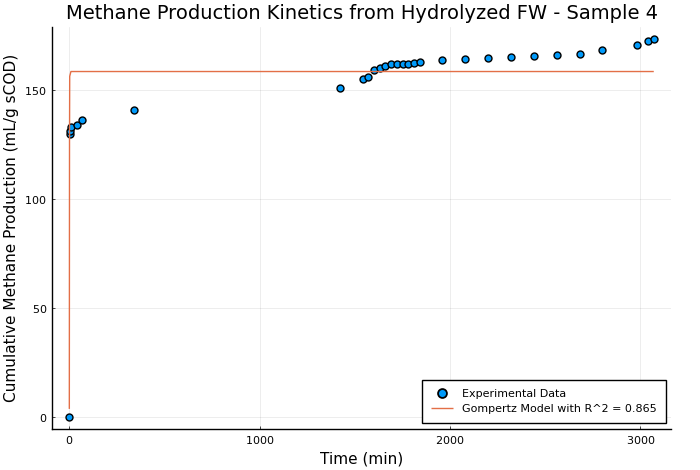
\includegraphics[width=.9\linewidth]{../plots/BMPs/Hydrolyzed FW/methane_kinetics_hydrolysate_4_min.png}
\end{center}

\begin{center}
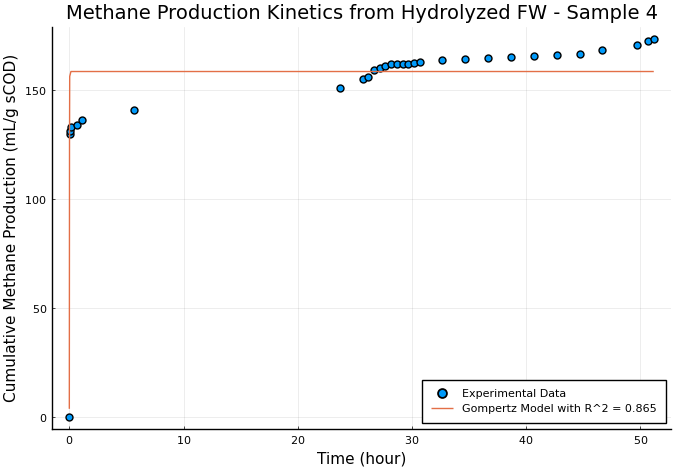
\includegraphics[width=.9\linewidth]{../plots/BMPs/Hydrolyzed FW/methane_kinetics_hydrolysate_4_hour.png}
\end{center}

\subsection{Untreated FW}
\label{sec:orgd195c81}
Εκτός από τα παραπάνω, σε ένα από τα δοχεία προστέθηκε ανεπεξέργαστο FW. Αυτό έχει διαφορά από το δείγμα 0, καθώς εκείνο υπέστει ζύμωση κατά τις 72 ώρες που ήταν στους 40 \(^oC\) ακόμη και χωρίς να προσθέσουμε κάποιο εμβόλιο, ενώ το δείγμα αυτό αναφέρεται σε food waste το οποίο δεν έχει υποστεί καμία επεξεργασία. Θα θέλαμε το δείγμα αυτό να έχει το χειρότερο performance (είτε πολύ αργή παραγωγή, ή μικρή τελική παραγωγή), το οποίο θα μας επιδείκνυε πως η επεξεργασία που έγινε βοηθάει πραγματικά στην χώνευση. Βέβαια, αξίζει να αναφερθεί πως το δοχείο αυτό είχε κάποιο προβλήματα με διαρροή στα αρχικά στάδια του πειράματος, οπότε ενδέχεται τα αποτελέσματα που θα προκύψουν να μην είναι έγκυρα. Παρακάτω φαίνεται ο κώδικας επεξεργασίας των αποτελεσμάτων του.

\textbf{untreated\textsubscript{fw}\textsubscript{1}\textsubscript{ad}}
\begin{minted}[breaklines=true,breakanywhere=true]{julia}

### Data Analysis on Untreated FW ###

<<date_saving_fw_1>>

inds = 12:34
exp_meth_vol = [0, 0.2, 0, 0.1, 0.1, 0, 0, 0, 0.1, 0.1, 0, 0.1, 0.2, 0.1, 0.1, 0.1, 0.0, 0.1, 0.2, 0.1, 0.2, 0.1, 0.1]
exp_name = "untreated_fw_1"
source = "Untreated FW"
sample = "FW 1"
input_cod = 0.1

<<bmp_data_processing>>

p0 = [20.0, 0.01, 1.0]
<<bmp_curve_fitting_min>>
model_hydro_fw_min = vcat(sample, model_params, r_squared)
<<bmp_data_plotting>>

p0 = [20.0, 1.0, 0.1]
<<bmp_curve_fitting_hour>>
model_hydro_fw_hour = vcat(sample, model_params, r_squared)
<<bmp_data_plotting>>
\end{minted}

\subsubsection{Results}
\label{sec:orgf358f63}
Το δείγμα αυτό παρήγαγε μόνο το \(7.1 \%\) του μεθανίου που είχε παράξει από οξικό και το έκανε αυτό σε έναν αργό σχετικά ρυθμό. Κρίνεται πιθανό να μην επιλύθηκαν τα προβλήματα διαρροής που είχε και η παραγωγή του αερίου να ήταν στην πραγματικότητα μεγαλύτερη. Όμως όπως και στο δείγμα με 0 ml ένζυμα το οποίο όμως υπέστει 3 μέρες υδρόλυση και ζύμωση, μας "βολεύει" τα ποσοστά αυτά να είναι πολύ χαμηλά επειδή σημαίνει πως η επεξεργασία που κάναμε όντως συνείσφερε στην παραγωγή μεθανίου.

Από άποψη προσαρμογής, το μοντέλο Gompertz μπορεί να προσαρμοστεί πολύ καλά σε τέτοια δεδομένα όπου η παραγωγή μεθανίου γίνεται σε παρόμοιο ρυθμό για όλη την διεργασία. Το μοντέλο που θα αντιστοιχήσει θα είναι ένα μοντέλο χαμηλού ρυθμού (με βάση την παραπάνω διάκριση), το οποίο όμως είναι το μόνο που μπορεί να ισχύει καθώς στην αρχή δεν υπάρχει μία απότομη παραγωγή αερίου ταχύτατα για να μπορεί να προσαρμοστεί κάτι διαφορετικό. Τα μοντέλα σε λεπτά και ώρες δεν προσαρμόζονται με τον ακριβώς ίδιο τρόπο, αλλά οι διαφορές τους είναι μικρές. Ο ειδικός ρυθμός ανάπτυξης είναι της τάξης του \(0.0137 \frac{ml}{g ~ sCOD \min} \text{ ή } 0.823 \frac{ml}{g ~ sCOD ~ hour}\). Τα άλλα μοντέλα που προσαρμόστηκαν με αργό ρυθμό ανάπτυξης είχαν κινητικές της τάξης του 0.03-0.05 \(\frac{ml}{g ~ sCOD \min }\) οπότε αυτό είναι πιο αργό αλλά συγκρίσιμο με εκείνα.

\begin{center}
\begin{tabular}{lrrrr}
Timestamp & Minutes & Hours & Methane\textsubscript{Volume} & Cumulative\textsubscript{Methane}\textsubscript{Volume}\\[0pt]
\hline
02/04\textsubscript{10}:54 & 0.0 & 0.0 & 0.0 & 0.0\\[0pt]
02/04\textsubscript{12}:54 & 120.0074 & 2.0001 & 0.2 & 0.2\\[0pt]
02/04\textsubscript{13}:24 & 150.0073 & 2.5001 & 0.0 & 0.2\\[0pt]
02/04\textsubscript{13}:54 & 180.0076 & 3.0001 & 0.1 & 0.3\\[0pt]
02/04\textsubscript{14}:24 & 210.0076 & 3.5001 & 0.1 & 0.4\\[0pt]
02/04\textsubscript{14}:54 & 240.0075 & 4.0001 & 0.0 & 0.4\\[0pt]
02/04\textsubscript{15}:24 & 270.0074 & 4.5001 & 0.0 & 0.4\\[0pt]
02/04\textsubscript{15}:54 & 300.0073 & 5.0001 & 0.0 & 0.4\\[0pt]
02/04\textsubscript{16}:24 & 330.0076 & 5.5001 & 0.1 & 0.5\\[0pt]
02/04\textsubscript{16}:54 & 360.0076 & 6.0001 & 0.1 & 0.6\\[0pt]
02/04\textsubscript{17}:24 & 390.0073 & 6.5001 & 0.0 & 0.6\\[0pt]
02/04\textsubscript{17}:54 & 420.0141 & 7.0002 & 0.1 & 0.7\\[0pt]
02/04\textsubscript{19}:54 & 540.0146 & 9.0002 & 0.2 & 0.9\\[0pt]
02/04\textsubscript{21}:54 & 660.0162 & 11.0003 & 0.1 & 1.0\\[0pt]
02/04\textsubscript{23}:54 & 780.0205 & 13.0003 & 0.1 & 1.1\\[0pt]
03/04\textsubscript{01}:54 & 900.0205 & 15.0003 & 0.1 & 1.2\\[0pt]
03/04\textsubscript{03}:54 & 1020.0203 & 17.0003 & 0.0 & 1.2\\[0pt]
03/04\textsubscript{05}:54 & 1140.0253 & 19.0004 & 0.1 & 1.3\\[0pt]
03/04\textsubscript{07}:54 & 1260.0272 & 21.0005 & 0.2 & 1.5\\[0pt]
03/04\textsubscript{09}:54 & 1380.0273 & 23.0005 & 0.1 & 1.6\\[0pt]
03/04\textsubscript{12}:54 & 1560.0362 & 26.0006 & 0.2 & 1.8\\[0pt]
03/04\textsubscript{13}:54 & 1620.036 & 27.0006 & 0.1 & 1.9\\[0pt]
03/04\textsubscript{14}:24 & 1650.037 & 27.5006 & 0.1 & 2.0\\[0pt]
\end{tabular}
\end{center}

\begin{center}
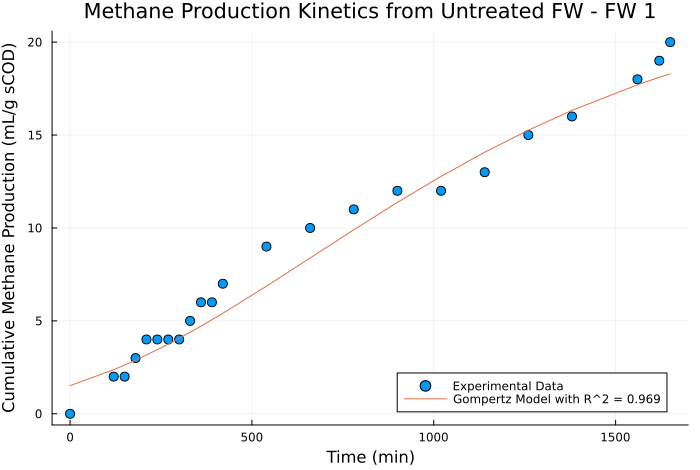
\includegraphics[width=.9\linewidth]{../plots/BMPs/Untreated FW/methane_kinetics_untreated_fw_1_min.png}
\end{center}

\begin{center}
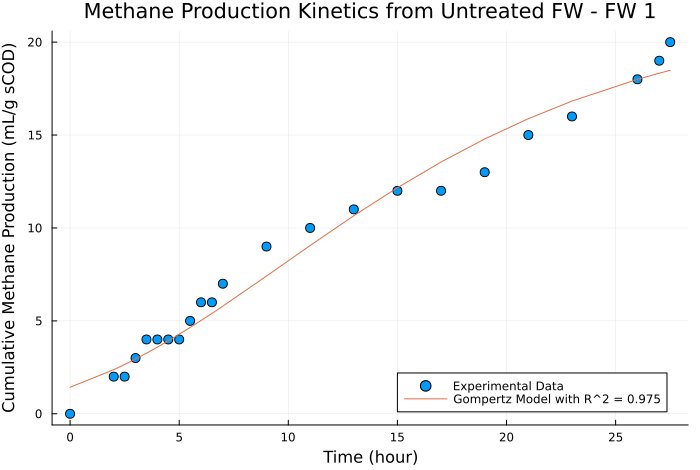
\includegraphics[width=.9\linewidth]{../plots/BMPs/Untreated FW/methane_kinetics_untreated_fw_1_hour.png}
\end{center}


\subsection{Update all}
\label{sec:org9c37242}
Όπως και παραπάνω για τα πειράματα στο οξικό, θα υπάρχει και ένα code block το οποίο θα κάνει update όλα τα code blocks, θα τα κάνει tangle σε ένα script file και θα αποθηκεύει ένα CSV με όλα τα κινητικά αποτελέσματα.

\textbf{update\textsubscript{hydrolysate}\textsubscript{tests}}
\begin{minted}[breaklines=true,breakanywhere=true]{julia}

<<hydrolysate_0_ad>>
<<hydrolysate_1_ad>>
<<hydrolysate_2_ad>>
<<hydrolysate_4_ad>>
<<untreated_fw_1_ad>>

model_fit_table_min = Tables.table(vcat(reshape(model_hydro_0_min, 1, 5), reshape(model_hydro_1_min, 1, 5), reshape(model_hydro_2_min, 1, 5), reshape(model_hydro_4_min, 1, 5), reshape(model_hydro_fw_min, 1, 5)), header = [:Sample_Name, :Methane_Production_Potential, :Methane_Production_Rate, :Lag_Time, :R_squared])
CSV.write(datadir("exp_pro", "methane_from_hydrolysate_kinetics_min.csv"), model_fit_table_min)

model_fit_table_hour = Tables.table(vcat(reshape(model_hydro_0_hour, 1, 5), reshape(model_hydro_1_hour, 1, 5), reshape(model_hydro_2_hour, 1, 5), reshape(model_hydro_4_hour, 1, 5), reshape(model_hydro_fw_hour, 1, 5)), header = [:Sample_Name, :Methane_Production_Potential, :Methane_Production_Rate, :Lag_Time, :R_squared])
CSV.write(datadir("exp_pro", "methane_from_hydrolysate_kinetics_hour.csv"), model_fit_table_hour)
\end{minted}

\begin{table}[htbp]
\caption{Kinetics with timescale in hours}
\centering
\begin{tabular}{lrrrr}
Sample\textsubscript{Name} & Production\textsubscript{Potential} & Production\textsubscript{Rate} & Lag\textsubscript{Time} & R2\\[0pt]
\hline
Sample 0 & 67.363 & 1.636 & 0.0 & 0.862\\[0pt]
Sample 1 & 163.745 & 3.175 & 0.0 & 0.815\\[0pt]
Sample 2 & 94.538 & 929.102 & 0.0404 & 0.724\\[0pt]
Sample 4 & 158.432 & 9732.61 & 0.00186 & 0.865\\[0pt]
FW 1 & 21.656 & 0.823 & 0.0 & 0.975\\[0pt]
\end{tabular}
\end{table}

\begin{table}[htbp]
\caption{Kinetics with timescale in minutes}
\centering
\begin{tabular}{lrrrr}
Sample\textsubscript{Name} & Production\textsubscript{Potential} & Production\textsubscript{Rate} & Lag\textsubscript{Time} & R2\\[0pt]
\hline
Sample 0 & 50.980 & 0.384 & 0.0 & 0.846\\[0pt]
Sample 1 & 105.569 & 0.840 & 0.0 & 0.689\\[0pt]
Sample 2 & 872.706 & 0.0320 & 0.0 & 0.687\\[0pt]
Sample 4 & 158.428 & 162.838 & 0.112 & 0.865\\[0pt]
FW 1 & 22.980 & 0.0127 & 0.0 & 0.969\\[0pt]
\end{tabular}
\end{table}
\end{document}
